% !TEX spellcheck=en_US
\documentclass[a4paper]{article}
\usepackage[american]{babel}
\usepackage[T1]{fontenc}
\usepackage[utf8]{inputenc}
\usepackage[activate={true,nocompatibility},final,tracking=true,kerning=true,spacing=true,factor=1100,stretch=10,shrink=10]{microtype}
\usepackage{graphicx}
\usepackage[table,dvipsnames]{xcolor}
\usepackage{caption}
\usepackage{subcaption}
\usepackage{csquotes}
\usepackage{hyperref}
\usepackage{url}
\usepackage[super]{nth}
\usepackage{amsmath}
\usepackage{amssymb}
\usepackage{amsthm}
\usepackage{mathtools}
\usepackage{mathmacros/mathmacros}
\usepackage{tcolorbox}
\usepackage{circuitikz}
\usepackage{tikz}
\usepackage{pgf}
\usepackage{pgfplots}
\usepackage[acronym]{glossaries}
\usepackage[backend=biber,style=phys]{biblatex}

% environments
\newtheorem{lemma}{Lemma}
\newtheorem{thm}{Theorem}
\newtheorem{crl}{Corollary}
\newtheorem{definition}{Definition}
\theoremstyle{remark}
\newtheorem{exm}{Example}
\theoremstyle{remark}
\newtheorem{rem}{Remark}

% misc macros
\newcommand*{\pref}[2]{#1 (\ref{#2})}
\definecolor{lightgray}{rgb}{0.9725,0.9725,0.9725}

% microtype
\SetTracking{encoding={*}, shape=sc}{0}

% pgfplots
\pgfplotsset{compat=newest}

\addbibresource{bibliography.bib}

\makenoidxglossaries
\newacronym{dne}{DNE}{does not exist}
\newacronym{wlog}{WLOG}{without loss of generality}

\begin{document}

\begin{titlepage}
	\centering
	{\scshape\Huge \bfseries{Advanced Systems} \par}
	\par\vspace{1cm}
	
\includegraphics[width=0.45\textwidth]{images/logo.png}\par
	\vspace{3cm}
	{\huge\bfseries Lecture Notes \par}
	\vspace{1cm}
	{\LARGE\itshape Mazawa Shinonome \par}
	\vspace{1cm}
	{\large\today\par}
	\vfill
	\begin{abstract}
		This document is a compilation of lecture notes for intermediate mathematics.
		It is intended to serve as a study guide for members of the Advanced System
		organization.
	\end{abstract}
\end{titlepage}

\newpage

\microtypesetup{protrusion=false}
\clearpage
\printnoidxglossaries
\newpage
\tableofcontents
\microtypesetup{protrusion=false}

\newpage

% === Begin Section Includes ===

\section{Acknowledgements}

TODO


\section{Introduction}

\begin{flushleft}
	The Advanced System organization is an open-source software community who's main
	purpose it is to develop modern and user-friendly utility programs. In order to
	develop advanced applications, the study of mathematics is of particular interests:
	It lays the groundwork for many other fields of studies such as physics or computer
	science.
\end{flushleft}

\begin{flushleft}
	While this document has been drafted with the best intents and purposes, there
	is no warranty on the correctness of its content. You can find the source code
	on \url{www.github.com/Advanced-Systems/lecture-notes} to compile a new PDF
	file from scratch using the most recent version of this document or raise an
	issue to report mistakes under the issues tab of GitHub.
\end{flushleft}


\section{Analysis}\label{sec-analysis}

TODO: Add description


\section{Logic}\label{sec-logic}

% ==============================================================================
% ==============================================================================
% ==============================================================================

\subsection{Truth Tables}\label{subsec-truth-table}

Propositional logic is a formal mathematical framework that encodes the truth value
of one or more propositions. A proposition is a statement that, by itself, is either
true or false. These propositions can be combined with binary operations to determine
the truth value of a statement expressed in the vernacular. While every proposition
is a statement, not every statement is a valid proposition.

\begin{enumerate}
    \item Questions are invalid propositions.
    \item Statements where the intention is unclear or ambiguous don't qualify as propositions, either.
\end{enumerate}

In practice, the variables \(A,B,C,\dots\) are often used to denote propositions.
Therefore, they are also sometimes referred to as \emph{propositional variables}
that can take on one of two possible values: \(T\) (true) or \(F\) (false). In
computer science, \(1\) (true) or \(0\) (false) are commonly used instead. It is
worth adding that many programming languages interpret any number \(n\neq0\) as
true\footnote{Take Python or C++ as prominent examples for this behavior.}. While
propositional logic has its place, inference systems are used in formal reasoning
instead, though this topic is beyond the scope of this subsection.

\begin{definition}\label{def-axiom}
    An axiom is a statement that is taken to be true and is confined within the
    system of logic they define. They establish the premise of reasoning and cannot
    be formally proved.
\end{definition}

There are five important axioms from which one can obtain a series of useful logical
statements that will later be used to formulate mathematical sound proofs. In order
to make this material more accessible, each axiom will be prefaced by a quote written
in the vernacular that accurately reflects the statement in question.

\begin{displayquote}
    ``\emph{It takes courage and strength to be empathetic.}''
    --- Jacinda Ardern\footnote{New Zealand politician who has been serving as the
    40th prime minister of New Zealand and leader of the Labour Party since 2017.}
\end{displayquote}

In this example, a person is said to be empathetic (\(C\)) if one is both
courageous (\(A\)) \emph{and} strong in character (\(B\)).

\begin{table}[hbt!]
    \centering
    \rowcolors{1}{}{lightgray}
    \begin{tabular}{*{6}{c}}
        $(A$ & $\land$ & $B)$ & $\rightarrow$ & $C$ \\
           T &         & T    &               & T   \\
           T &         & F    &               & T   \\
           F &         & T    &               & F   \\
           F &         & F    &               & F   \\
    \end{tabular}
    \caption{Conjunction}\label{table-conjunction}
\end{table}

\begin{displayquote}
    ``\emph{So much of life is not about whether you're good or bad, or right or
    wrong, or can afford or not afford -- it's about timing.}''
    -- Adrian Anthony Gill\footnote{Scottish writer and critic.}
\end{displayquote}

In natural languages, a distinction is often drawn implicitly between inclusive
and exclusive disjunctions. See \pref{table}{table-disjunction} as an example of
the inclusive disjunction (\emph{or}). The truth table for the exclusive disjunction
(\emph{xor}) will be introduced later in \pref{subsection}{subsec-circuit-representation}.

\begin{table}[hbt!]
    \centering
    \rowcolors{1}{}{lightgray}
    \begin{tabular}{*{6}{c}}
        $(A$ & $\lor$ & $B)$ & $\rightarrow$ & $C$ \\
           T &        & T    &               & T   \\
           T &        & F    &               & T   \\
           F &        & T    &               & T   \\
           F &        & F    &               & F   \\
    \end{tabular}
    \caption{Disjunction}\label{table-disjunction}
\end{table}

\begin{displayquote}
    ``\emph{'Awkward' implies both solidarity and implication. Nobody is exempt.}''
    -- Elif Batuman\footnote{American author, academic, and journalist.}
\end{displayquote}

One interesting thing to note about \pref{table}{table-subjunction} is that it is
possible to arrive to true statements even if the premise or assumption turned out
to be incorrect, an important implication of this being that there are no valuable
insights to be gained from a false premise. Therefore, it is of utmost importance
in logical reasoning to verify that the starting arguments have a positively affirmative
truth value.

\begin{table}[hbt!]
    \centering
    \rowcolors{1}{}{lightgray}
    \begin{tabular}{*{6}{c}}
        $(A$ & $\Rightarrow$ & $B)$ & $\rightarrow$ & $C$ \\
           T &               & T    &               & T   \\
           T &               & F    &               & F   \\
           F &               & T    &               & T   \\
           F &               & F    &               & T   \\
    \end{tabular}
    \caption{Subjunction}\label{table-subjunction}
\end{table}

\begin{displayquote}
    ``\emph{One man is equivalent to all Creation. One man is a World in miniature.}''
    -- Albert Pike\footnote{American author, poet, orator, editor, lawyer, jurist,
    and prominent member of the Freemasons}
\end{displayquote}

Logically equivalent statements share the same truth value across all occurring
propositional variables. They become important later in ring proofs where multiple
distinct propositions implicate each other in all directions.

\begin{table}[hbt!]
    \centering
    \rowcolors{1}{}{lightgray}
    \begin{tabular}{*{6}{c}}
        $(A$ & $\Leftrightarrow$ & $B)$ & $\rightarrow$ & $C$ \\
           T &                   & T    &               & T   \\
           T &                   & F    &               & F   \\
           F &                   & T    &               & F   \\
           F &                   & F    &               & T   \\
    \end{tabular}
    \caption{Bisubjunction}\label{table-bisubjunction}
\end{table}

\begin{exm}\label{exm-logical-equivalent}
    It is left to the reader as an exercise to use a truth table to verify the
    following proposition:
    \begin{equation}
        \left((A \Rightarrow B) \land (B \Rightarrow A)\right) \Leftrightarrow (A \Leftrightarrow B)
    \end{equation}
\end{exm}

\begin{displayquote}
    ``\emph{No worse fate can befall a young man or woman than becoming prematurely
    entrenched in prudence and negation.}''
    -- Knut Hamsun\footnote{Norwegian writer and Nobel Prize winner in Literature
    in 1920.}
\end{displayquote}

Negation is one of the simplest unary operations in that it inverts the truth
value of a propositional variable.

\begin{table}[hbt!]
    \centering
    \rowcolors{1}{}{lightgray}
    \begin{tabular}{*{6}{c}}
        $(\neg B)$ & $\rightarrow$ & $C$ \\
                 T &               & F   \\
                 F &               & T   \\
    \end{tabular}
    \caption{Negation}\label{table-negation}
\end{table}

% ==============================================================================
% ==============================================================================
% ==============================================================================

\subsection{Circuit Representation of Logical Operations}\label{subsec-circuit-representation}

Truth tables are very useful in determining the nature of logic gates.
In \pref{table}{subsec-truth-table} find defined the axioms which build the basis for
this section. Take \texttt{XOR}, for instance: this logic gate evaluates to $1$
if and only if one of both poles receives $1$ as an input as opposed to \texttt{OR}
which also accepts two positive-valued states favorably.

\begin{table}[hbt!]
    \centering
    \rowcolors{1}{}{lightgray}
    \begin{tabular}{*{6}{c}}
        $A$ & $B$ & $A\texttt{ OR }B$ & $A\texttt{ AND }B$ & $A\texttt{ NAND }B$ & $(A\texttt{ OR }B)\texttt{ AND }(A\texttt{ NAND }B)$ \\
          1 & 1   & 1                 & 1                  & 0                   & 0                                                    \\
          1 & 0   & 1                 & 0                  & 1                   & 1                                                    \\
          0 & 1   & 1                 & 0                  & 1                   & 1                                                    \\
          0 & 0   & 0                 & 0                  & 1                   & 0                                                    \\
    \end{tabular}
    \caption{\texttt{XOR} Truth Table}\label{truth-table-xor}
\end{table}

Based on this truth table it is possible to implement a logic gate that replicates
a \texttt{XOR} gate in the following way:

\begin{figure}[hbt!]
    \centering
    \begin{circuitikz}
        % gates
        \node[or port,draw] at (0,2) (or) {};
        \node[nand port,draw] at (0,0) (nand) {};
        \node[and port,draw] at (2,1) (and) {};
        % inputs
        \node at ($(or.in 1) + (-1,0)$) (A) {$A$};
        \node at ($(nand.in 2) + (-1,0)$) (B) {$B$};
        % wires
        \draw (A) -- (or.in 1);
        \draw (A) -- (nand.in 1);
        \draw (B) -- (or.in 2);
        \draw (B) -- (nand.in 2);
        \draw (or.out) -- (and.in 1);
        \draw (nand.out) -- (and.in 2);
        \draw (and.out) -- ($(and.out) + (0.5,0)$) node[anchor=west] (Q) {$Q$};
    \end{circuitikz}
    \caption{Circuit of an \texttt{XOR} gate}\label{circuit-xor-gate}
\end{figure}

A half adder is a circuit that adds two binary numbers, each one bit in size.
The result $S$ is also represented by a one bit value, so in case of 
$1_2+1_2=(10)_2$ the second digit must be carried over in $C$ (hence the name 
\textit{carrier}) in order to be preserved for future operations.

\begin{figure}[hbt!]
    \centering
    \begin{circuitikz}
        % xor gate
        \node[xor port,draw] at (0,2) (xor) {};
        \draw (xor.in 1) -- ($(xor.in 1) + (-0.75,0)$) node[anchor=east] (A) {$A$};
        \draw (xor.in 2) -- ($(xor.in 2) + (-0.75,0)$) node[anchor=east] (B) {$B$};
        \draw (xor.out) -- ($(xor.out) + (0.75,0)$) node[anchor=west] (S) {$S$};
        % and gate   
        \node[and port,draw] at (0,0) (and) {};
        \draw (xor.in 1) -- (and.in 1);
        \draw ($(xor.in 2) + (-0.25,0)$) -- ($(and.in 2) + (-0.25,0)$) -- (and.in 2);
        \draw (and.out) -- ($(and.out) + (0.75,0)$) node[anchor=west] (C) {$C$};        
    \end{circuitikz}
    \caption{Circuit of an half adder}\label{circuit-half-adder}
\end{figure}

\begin{table}[hbt!]
    \centering
    \rowcolors{1}{}{lightgray}
    \begin{tabular}{*{4}{c}}
        $A$ & $B$ & $S$ & $C$ \\
          1 & 1   & 0  & 1    \\
          1 & 0   & 1  & 0    \\
          0 & 1   & 1  & 0    \\
          0 & 0   & 0  & 0    \\
    \end{tabular}
    \caption{Half Adder Truth Table}\label{truth-table-half-adder}
\end{table}

As opposed to an half adder, a full adder takes one more input (a so-called \texttt{carry in})
and two outputs, \textit{i.e.} \texttt{carry out} and \texttt{sum}. To build a
more sophisticated adder, chain half adders in a way that allows the result of
the previous sum to be carried over as \texttt{cin} to the next half adder.

\begin{figure}[hbt!]
    \centering
    \begin{circuitikz}
        % gates
        \node[xor port,draw,anchor=center] at (0,4) (xor1) {D};
        \node[xor port,draw] at (2,4) (xor2) {};
        \node[and port,draw] at (2,2) (and1) {E};
        \node[and port,draw] at (2,0) (and2) {F};
        \node[or port,draw] at (4,1) (or) {};
        % inputs
        \node at ($(xor1.in 1) + (-1,0)$) (A) {$A$};
        \node at ($(xor1.in 2) + (-1,0)$) (B) {$B$};
        \node at ($(A) + (0,-1.5)$) (C) {$C_{in}$};
        % wires
        \draw (A) -- (xor1.in 1);
        \draw (B) -- (xor1.in 2);
        \draw (xor1.out) -- (xor2.in 1);
        \draw (C) -- (xor2.in 2);
        \draw (C) -- (and1.in 1);
        \draw (xor1.out) -- ($(and1.in 2)-(0.5,0)$) -- (and1.in 2);
        \draw ($(A)+(0.75,0)$) -- ($(A)+(0.75,-4.56)$) -- (and2.in 2);
        \draw ($(B)+(1,0)$) -- ($(B)+(1,-3.425)$) -- (and2.in 1);
        \draw (and1.out) -- (or.in 1);
        \draw (and2.out) -- (or.in 2);
        \draw (xor2.out) -- ($(xor2.out) + (0.5,0)$) node[anchor=west] (S) {$S$};
        \draw (or.out) -- ($(or.out) + (0.5,0)$) node[anchor=west] (Q) {$C_{out}$};
    \end{circuitikz}
    \caption{Circuit of an full adder}\label{circuit-full-adder:1}
\end{figure}

Circuit \pref{figure}{circuit-full-adder:1} introduced three additional truth values 
to make the truth \pref{table}{truth-table-full-adder} for the full adder easier
to read\footnote{Note that $S:\Leftrightarrow D\texttt{ XOR } C_{in}$ and 
$C_{out} :\Leftrightarrow E\texttt{ OR }F$}. It is helpful to think of gate $D$
and gate $F$ as the first half adder.

\begin{table}[hbt!]
    \centering
    \rowcolors{1}{}{lightgray}
    \begin{tabular}{*{8}{c}}
        $A$ & $B$ & $C_{in}$ & $A\texttt{ XOR }B$ & $D\texttt{ XOR }C_{in}$ & $D\texttt{ AND }C_{in}$ & $F$ & $E\texttt{ OR }F$ \\
          1 & 1   & 1        & 0                  & 1                       & 0                       & 1   & 1                 \\
          1 & 1   & 0        & 0                  & 0                       & 0                       & 1   & 1                 \\
          1 & 0   & 1        & 1                  & 0                       & 1                       & 0   & 1                 \\
          0 & 1   & 1        & 1                  & 0                       & 1                       & 0   & 1                 \\
          1 & 0   & 0        & 1                  & 1                       & 0                       & 0   & 0                 \\
          0 & 1   & 0        & 1                  & 1                       & 0                       & 0   & 0                 \\
          0 & 0   & 1        & 0                  & 1                       & 0                       & 0   & 0                 \\
          0 & 0   & 0        & 0                  & 0                       & 0                       & 0   & 0                 \\
    \end{tabular}
    \caption{Full Adder Truth Table}\label{truth-table-full-adder}
\end{table}


\subsection{Sets}\label{subsec-sets}

% ==============================================================================
% ==============================================================================
% ==============================================================================

TODO: Add description

\subsubsection{Indicator Functions}\label{subsubsec-indicator-functions}

\begin{definition}\label{def-indicator-function}
	Let $X$ be a set. For each subset $A \subseteq X$ there is defined the
	indicator function\footnote{Sometimes, the term characteristic function is
		used to describe the function that indicates membership in a set in other
		fields of mathematics. The term indicator function is more prominently used
		in probability theory.} $\chi_A:X\rightarrow \{0,1\}$ of the set $A$ as
	\begin{equation}
		\chi_A(x) = \begin{cases}
			1,\;\text{ if } x \in A \\
			0,\;\text{ if } x \notin A
		\end{cases}
	\end{equation}
	We will write $\chi_A$ instead of $\chi_A(x)$ if the parameter
	$x$ is unambiguous.
\end{definition}

\begin{thm}\label{thm-complement-indicator-function}
	Let $\chi_A$ be an indicator function. Then the complement of $A$ (i.e.
	$\overline{A} \defines A^C$) is
	\begin{equation*}
		\chi_{\overline{A}} = 1 - \chi_A
	\end{equation*}
\end{thm}

\begin{proof}
	Of \pref{theorem}{thm-complement-indicator-function}.
	\begin{align*}
		\chi_{\overline{A}}(x) & = \begin{cases}
			1,\;\text{ if } \neg(x \in A) \\
			0,\;\text{ if } \neg(x \notin A)
		\end{cases}    \\
		                       & = \begin{cases}
			1-0,\;\text{ if } x \notin A \\
			1-1,\;\text{ if } x \in A
		\end{cases}    \\
		                       & =1 - \begin{cases}
			0,\;\text{ if } x \notin A \\
			1,\;\text{ if } x \in A
		\end{cases} \\
		                       & = 1 - \chi_A(x)
	\end{align*}
\end{proof}

\begin{thm}\label{thm-set-cardinality-indicator-function}
	Let $\chi_A$ be an indicator function with $A$ as a finite set. Then,
	\begin{equation*}
		\abs{A} = \sum_{x \in X} \chi_A(x)
	\end{equation*}
\end{thm}

\begin{proof}
	Of theorem (\ref{thm-set-cardinality-indicator-function}).
	\begin{align*}
		\abs{A} & =\sum_{x\in A}\underbrace{\chi_A(x)}_{1}                                   \\
		        & =\sum_{x\in A}\chi_A(x)+\sum_{x\in X\setminus A}\underbrace{\chi_A(x)}_{0} \\
		        & =\sum_{x\in (A\cup (X\setminus A))}\chi_A(x)                               \\
		        & \overset{(\star)}{=}\sum_{x\in X}\chi_A(x).
	\end{align*}
	since
	\begin{equation*}
		(\star) :\Leftrightarrow A\cup(X\setminus A)=(A\cup X)\setminus(A\setminus A)=X\setminus \emptyset=X
	\end{equation*}
\end{proof}

\begin{thm}\label{thm-cap-indicator-function}
	Let $\chi_A,\chi_B$ be indicator functions. Then:
	\begin{equation*}
		\chi_{A \cap B} = \chi_A\chi_B
	\end{equation*}
\end{thm}

\begin{proof}
	Of \pref{theorem}{thm-cap-indicator-function}.
	\begin{align*}
		\chi_{A \cap B} & = \begin{cases}
			1\;\text{ if } x \in (A \cap B) \\
			0\;\text{ if } x \notin (A \cap B)
		\end{cases}                                                     \\
		                & = \begin{cases}
			1\;\text{ if } x \in A \land x \in B \\
			0\;\text{ if } x \notin A \land x \notin B
		\end{cases}                                                     \\
		                & = \left(\begin{cases}
				1\;\text{ if } x \in A \\
				0\;\text{ if } x \notin A
			\end{cases}\right)\left(\begin{cases}
				1\;\text{ if } x \in B \\
				0\;\text{ if } x \notin B
			\end{cases}\right) \\
		                & = \chi_A\chi_B
	\end{align*}
\end{proof}

\begin{thm}\label{thm-cup-indicator-function}
	Let $\chi_A,\chi_B$ be indicator functions. Then:
	\begin{equation*}
		\chi_{A \cup B} = \chi_A + \chi_B - \chi_A\chi_B
	\end{equation*}
\end{thm}

\begin{proof}
	Of \pref{theorem}{thm-cup-indicator-function}.
	By using the fact that $\overline{\overline{A}}=A$ in combination with
	\pref{theorem}{thm-complement-indicator-function} and
	\pref{theorem}{thm-cap-indicator-function} we get that
	\begin{align*}
		\chi_{\overline{\overline{A \cup B}}}
		 & = 1 - \chi_{\overline{A \cup B}}                               \\
		 & \overset{(\star)}{=} 1 - \chi_{\overline{A} \cap \overline{B}} \\
		 & = 1 - \chi_{\overline{A}} \chi_{\overline{B}}                  \\
		 & = 1 - (1 - \chi_A)(1 - \chi_B)                                 \\
		 & = 1 - \left(1 - \chi_B - \chi_A + \chi_A\chi_B\right)          \\
		 & = \chi_A - \chi_B + \chi_A\chi_B                               \\
	\end{align*}
	Recall that $(\star)$ uses one of De Morgan's laws which states that
	\begin{align*}
		(\star) & \iff \overline{A \cup B}                             \\
		        & \iff \bigwedge_{x\in X}\{x\notin (A\cup B)\}         \\
		        & \iff \bigwedge_{x\in X}\{x\notin A \land x\notin B\} \\
		        & \iff \overline{A} \cap \overline{B}
	\end{align*}
\end{proof}


\subsection{Functions}\label{subsec-functions}

\begin{definition}\label{def-function}
	Let $M,N$ be two sets. A subset $F \subset M \times N$ is called a function
	from $M$ to $N$ if \cite[p.27]{wuest2009}
	\begin{equation}
		(\left<x,y\right> \in F \land \left<x,z\right> \in F)
		\implies y = z \quad (x \in M,\:y,z \in N)
	\end{equation}
\end{definition}

\begin{definition}\label{def-domain-range}
	Let $F \subset M \times N$ be a function. The sets
	\begin{align}
		\domain{F}   & = \left\{x \setbuild x \in M \text{ there exists } y \in N \text{ with } \left<x,y\right> \in F \right\} \label{def-domain}   \\
		\codomain{F} & = \left\{y \setbuild y \in N \text{ there exists } x \in M \text{ with } \left<x,y\right> \in F \right\} \label{def-codomain}
	\end{align}
	are called domain and codomain, respectively.
\end{definition}

\begin{figure}[ht!]
	\centering
	\begin{tikzpicture}
		% center rectangle
		\draw [color=black,dashed] (0,0) rectangle (6,4) node[above] {$X \times Y$};
		\draw [color=red,very thick] (1,1) to[out=-45,in=180] (5,3) node[below,anchor=south east] {$F\subset M \times N$};
		% horizontal bar
		\draw [color=MidnightBlue,very thick] (0,-1) -- (6,-1) node[anchor=north east] {$X$};
		\draw [color=BurntOrange,very thick] (1,-1) -- (5,-1) node[anchor=north east] {$F^{-1}(N)$};
		\draw [color=BurntOrange,dashed] (1,-1) -- (1,1);
		\draw [color=BurntOrange,dashed] (5,-1) -- (5,3);
		% vertical bar
		\draw [color=DarkOrchid,very thick] (-1,0) -- (-1,4) node[anchor=north east] {$Y$};
		\draw [color=ForestGreen,very thick] (-1,1) -- (-1,3) node[anchor=north east] {$F(M)$};
		\draw [color=ForestGreen,dashed] (-1,1) -- (1,1);
		\draw [color=ForestGreen,dashed] (-1,3) -- (5,3);
	\end{tikzpicture}
	\caption{Graphical depiction of a valid sample function}
	\label{sketch-valid-function}
\end{figure}

\begin{flushleft}
	If $\domain{F}\subset M$ with $F$ as a well defined function, we will use the
	the following shorthand notations as is customary:
	\begin{align*}
		F:\;           & \mathcal{D} \rightarrow N                \\
		               & x\mapsto F(x)                            \\\\
		\text{or}\quad & F:x\mapsto F(x)\qquad{(x\in\mathcal{D})} \\\\
		\text{or}\quad & F:y=F(x)\qquad{(x\in\mathcal{D})}
	\end{align*}
\end{flushleft}

\begin{definition}\label{def-image-preimage}
	Let $F : X \rightarrow Y$ be a function where $M\subseteq X$ and $N \subseteq Y$.
	Then
	\begin{align}
		F(M)      & \defines \left\{F(x) \setbuild x \in M \right\}\subseteq Y \label{eq-image} \\
		F^{-1}(N) & \defines \left\{x \in X \setbuild F(x) \in N \right\}\label{eq-preimage}
	\end{align}
	are called the image\footnote{Alternative notation: $\text{Im}(F)$} of $M$
	under $F$ and the preimage\footnote{Urbild (\textit{German})} of $F$ under $N$, respectively
	\cite[p.16]{liesenMehrmann2015}.
\end{definition}

\begin{rem}
	The domain can be any arbitrary set that makes sense for a function $F$ (e.g.
	don't allow dividing by zero). The image is the set of all possible values the
	function can actually take on. Often the codomain is equal to the image of a
	function, but in some instances this is not the case. For example,
	\begin{align*}
		F(x):\mathbb{R}\rightarrow\mathbb{R},x\mapsto x^2
	\end{align*}
	In this example $F(x)\defines x^2$ can never take on any negative numbers,
	so the image of $F$ is $F(\mathbb{R})=[0,\infty)\subset\domain{F}$. This
	function never assumes any negative numbers which clearly also belong to the
	set of real numbers. On the other hand, the preimage of the image should be
	the whole domain. Each subset of the image has a preimage that can be considered
	separately, e.g. $ F^{-1}(\{4,9\})=\{-3,-2,2,3\}$.
\end{rem}

\begin{figure}[ht!]
	\centering
	\begin{tikzpicture}
		% center rectangle
		\draw [color=black,dashed] (0,0) rectangle (6,4) node[above] {$X \times Y$};
		\draw [color=red,very thick] (1,1) to[out=-50,in=20] (1,3) node[below,anchor=south west] {$F\subset M \times N$};
		% horizontal bar
		\draw [color=MidnightBlue,very thick] (0,-1) -- (6,-1) node[anchor=north east] {$X$};
		\draw [color=BurntOrange,very thick] (1,-1) -- (5,-1) node[anchor=north east] {$F^{-1}(N)$};
		\draw [color=BurntOrange,dashed] (1,-1) node[anchor=south west] {$x$} -- (1,3);
		% vertical bar
		\draw [color=DarkOrchid,very thick] (-1,0) -- (-1,4) node[anchor=north east] {$Y$};
		\draw [color=ForestGreen,very thick] (-1,1) -- (-1,3) node[anchor=north east] {$F(M)$};
		\draw [color=ForestGreen,dashed] (-1,1) node[anchor=north west] {$y_1$} -- (1,1);
		\draw [color=ForestGreen,dashed] (-1,3) node[anchor=north west] {$y_2$} -- (1,3);
	\end{tikzpicture}
	\caption{Example of what constitutes a violation of \pref{definition}{def-function}}
	\label{sketch-invalid-function}
\end{figure}

\begin{definition}
	Let $F \subset M \times N$ be a function from $M$ to $N$ $:\Leftrightarrow \domain{F}=M$.
	Then for $x_1,x_2\in M, y\in N$:
	\begin{itemize}
		\item $F$ surjective $:\Leftrightarrow\codomain{F}=N$\label{def-surjective}
		\item $F$ injective $:\Leftrightarrow(\left<x_1,y\right>\in F \land \left<x_2,y\right>\in F)\implies x_1=x_2$\label{def-injective}
		\item $F$ bijective $:\Leftrightarrow$ $F$ surjective and injective \label{def-bijective}
	\end{itemize}
\end{definition}

\begin{exm}\label{exm-injective-function}
	Let $f:\mathbb{R}\rightarrow\mathbb{R},f(x)=2x+3$. Is this function injective?
	\begin{flushleft}
		\textbf{Answer}: Suppose there are two values $x_1,x_2\in\mathbb{R}$ such
		that $f(x_1)=f(x_2)$. Then
		\begin{align*}
			f(x_1)          & = f(x_2) \\
			\implies 2x_1+3 & = 2x_2+3 \\
			\implies   2x_1 & = 2x_2   \\
			\implies    x_1 & = x_2
		\end{align*}
		Therefore the function $f(x)=2x+3$ is injective. With respect to
		\pref{figure}{sketch-injective-function} this means that every value from
		the codomain is taken on \textit{at most} once.
	\end{flushleft}
	\begin{rem}
		In order to determine whether a function is injective
		or not assume that there exists an $x_1,x_2$ where $x_1 \neq x_2$ such
		that $f(x_1)=f(x_2)$. If you can show that this is only true for $x_1=x_2$
		then you are done, if not then the function is not injective.
	\end{rem}
\end{exm}

\begin{figure}[ht!]
	\centering
	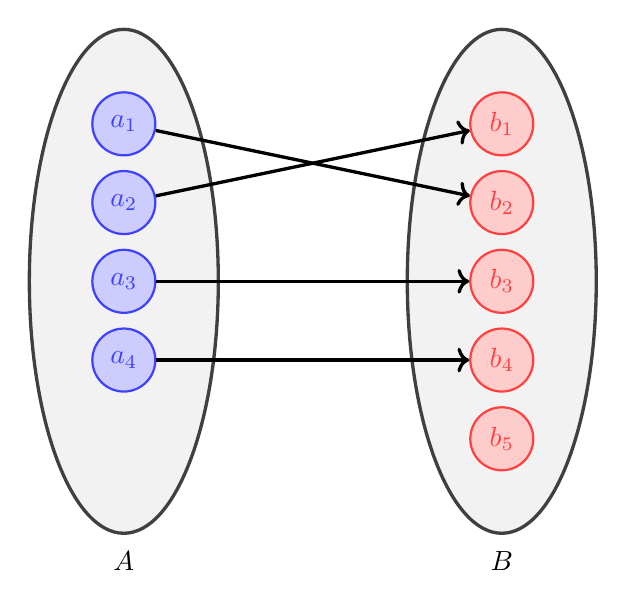
\begin{tikzpicture}[scale=0.8]
		\tikzstyle{blue-node}=[color=blue!75,fill=blue!20,thick,circle, draw, minimum width=0.8cm]
		\tikzstyle{red-node}=[color=red!75,fill=red!20,thick,circle, draw, minimum width=0.8cm]
		\tikzstyle{parent}=[color=black!75,fill=black!5,very thick]
		\tikzstyle{mapsto}=[->,very thick]
		% set A
		\draw [parent] (-2,0) ellipse (1.5cm and 4cm);
		\node [blue-node] at (-2,2.5) (a1) {$a_1$};
		\node [blue-node] at (-2,1.25) (a2) {$a_2$};
		\node [blue-node] at (-2,0) (a3) {$a_3$};
		\node [blue-node] at (-2,-1.25) (a4) {$a_4$} (-2,-4.75) node[anchor=south,color=black] {$A$};
		% set B
		\draw [parent] (4,0) ellipse (1.5cm and 4cm);
		\node [red-node] at (4,2.5) (b1) {$b_1$};
		\node [red-node] at (4,1.25) (b2) {$b_2$};
		\node [red-node] at (4,0)(b3) {$b_3$};
		\node [red-node] at (4,-1.25) (b4) {$b_4$};
		\node [red-node] at (4,-2.5) (b5) {$b_5$} (4,-4.75) node[anchor=south,color=black] {$B$};
		% mapsto
		\draw [mapsto] (a1) -- (b2);
		\draw [mapsto] (a2) -- (b1);
		\draw [mapsto] (a3) -- (b3);
		\draw [mapsto] (a4) -- (b4);
	\end{tikzpicture}
	\caption{Example of an injective function}
	\label{sketch-injective-function}
\end{figure}

\begin{exm}\label{exm-surjective-function}
	Let $f:\mathbb{R}\rightarrow\mathbb{R},f(x)=2x+3$. Is this function surjective?
	\begin{flushleft}
		\textbf{Answer}: For any $y=f(x)\in\mathbb{R}$ there exists an $x=\frac{y-3}{2}$
		such that
		\begin{align*}
			f(x) & = 2\left(\frac{y-3}{2}\right)+3 \\
			     & = y - 3 + 3                     \\
			     & = y
		\end{align*}
		This proves that the function $f(x)=2x+3$ is surjective since $\text{Im}(f)=\mathbb{R}$.
		With respect to \pref{figure}{sketch-surjective-function} this means that
		every value from the codomain is taken on \textit{at least} once.
	\end{flushleft}
	\begin{rem}
		The strategy for determining whether a function is
		surjective or not boils down to solving the original function definition
		for $x$ and plugging in this expression in $f(x)$. If you can show that
		$f(x)=y$ then you are done, if not then the function is not surjective.
	\end{rem}
\end{exm}

\begin{figure}[ht!]
	\centering
	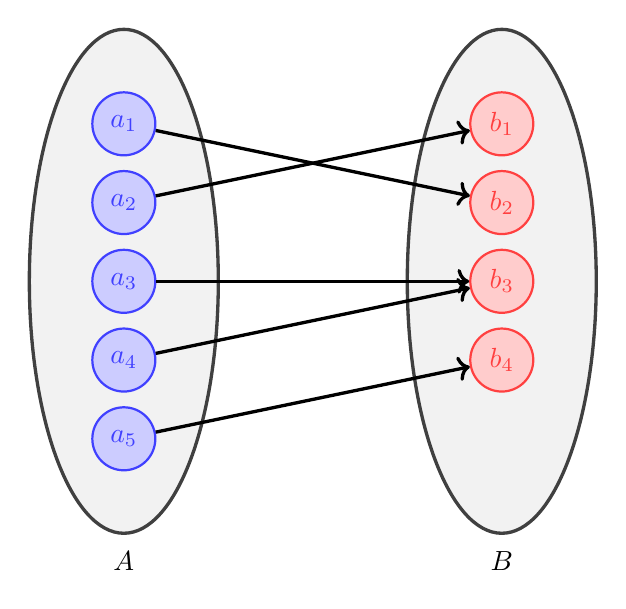
\begin{tikzpicture}[scale=0.8]
		\tikzstyle{blue-node}=[color=blue!75,fill=blue!20,thick,circle, draw, minimum width=0.8cm]
		\tikzstyle{red-node}=[color=red!75,fill=red!20,thick,circle, draw, minimum width=0.8cm]
		\tikzstyle{parent}=[color=black!75,fill=black!5,very thick]
		\tikzstyle{mapsto}=[->,very thick]
		% set A
		\draw [parent] (-2,0) ellipse (1.5cm and 4cm);
		\node [blue-node] at (-2,2.5) (a1) {$a_1$};
		\node [blue-node] at (-2,1.25) (a2) {$a_2$};
		\node [blue-node] at (-2,0) (a3) {$a_3$};
		\node [blue-node] at (-2,-1.25) (a4) {$a_4$};
		\node [blue-node] at (-2,-2.5) (a5) {$a_5$} (-2,-4.75) node[anchor=south,color=black] {$A$};
		% set B
		\draw [parent] (4,0) ellipse (1.5cm and 4cm);
		\node [red-node] at (4,2.5) (b1) {$b_1$};
		\node [red-node] at (4,1.25) (b2) {$b_2$};
		\node [red-node] at (4,0)(b3) {$b_3$};
		\node [red-node] at (4,-1.25) (b4) {$b_4$} (4,-4.75) node[anchor=south,color=black] {$B$};
		% mapsto
		\draw [mapsto] (a1) -- (b2);
		\draw [mapsto] (a2) -- (b1);
		\draw [mapsto] (a3) -- (b3);
		\draw [mapsto] (a4) -- (b3);
		\draw [mapsto] (a5) -- (b4);
	\end{tikzpicture}
	\caption{Example of an surjective function}
	\label{sketch-surjective-function}
\end{figure}

\begin{exm}\label{exm-bijective-function}
	Let $f:\mathbb{R}\rightarrow\mathbb{R},f(x)=2x+3$. Is this function bijective?
	\begin{flushleft}
		\textbf{Answer}: From \pref{example}{exm-injective-function} and
		\pref{example}{exm-surjective-function} we can deduce that since the function
		is injective and surjective, that it is bijective as well. With respect
		to \pref{figure}{sketch-bijective-function} this means that every value
		from the codomain is taken on \textit{exactly} once.
	\end{flushleft}
\end{exm}

\begin{figure}[ht!]
	\centering
	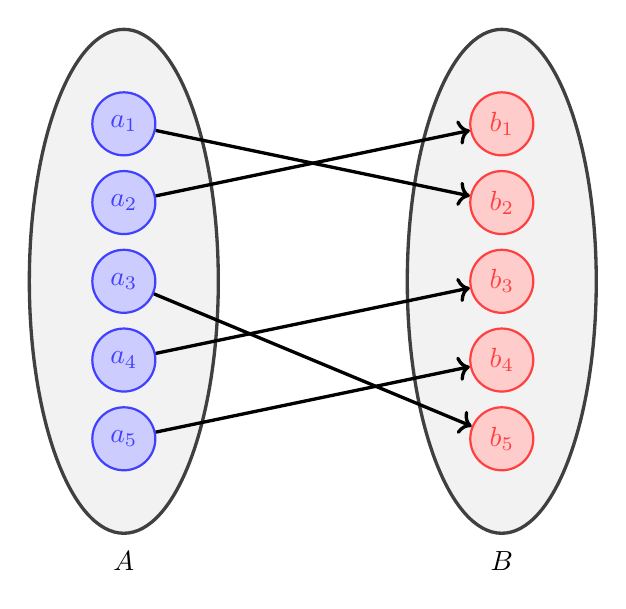
\begin{tikzpicture}[scale=0.8]
		\tikzstyle{blue-node}=[color=blue!75,fill=blue!20,thick,circle, draw, minimum width=0.8cm]
		\tikzstyle{red-node}=[color=red!75,fill=red!20,thick,circle, draw, minimum width=0.8cm]
		\tikzstyle{parent}=[color=black!75,fill=black!5,very thick]
		\tikzstyle{mapsto}=[->,very thick]
		% set A
		\draw [parent] (-2,0) ellipse (1.5cm and 4cm);
		\node [blue-node] at (-2,2.5) (a1) {$a_1$};
		\node [blue-node] at (-2,1.25) (a2) {$a_2$};
		\node [blue-node] at (-2,0) (a3) {$a_3$};
		\node [blue-node] at (-2,-1.25) (a4) {$a_4$};
		\node [blue-node] at (-2,-2.5) (a5) {$a_5$} (-2,-4.75) node[anchor=south,color=black] {$A$};
		% set B
		\draw [parent] (4,0) ellipse (1.5cm and 4cm);
		\node [red-node] at (4,2.5) (b1) {$b_1$};
		\node [red-node] at (4,1.25) (b2) {$b_2$};
		\node [red-node] at (4,0)(b3) {$b_3$};
		\node [red-node] at (4,-1.25) (b4) {$b_4$};
		\node [red-node] at (4,-2.5) (b5) {$b_5$} (4,-4.75) node[anchor=south,color=black] {$B$};
		% mapsto
		\draw [mapsto] (a1) -- (b2);
		\draw [mapsto] (a2) -- (b1);
		\draw [mapsto] (a3) -- (b5);
		\draw [mapsto] (a4) -- (b3);
		\draw [mapsto] (a5) -- (b4);
	\end{tikzpicture}
	\caption{Example of an bijective function}
	\label{sketch-bijective-function}
\end{figure}

\begin{exm}\label{exm-injective-surjective-bijective}
	Determine whether the following functions are injective, surjective or
	bijective\footnote{You may also consult \pref{figure}{sktech:exm-1:4} for
		additional help.}:
	\begin{enumerate}
		\item[1.)] $f(x):\mathbb{R}^+\rightarrow\mathbb{R}^+,x\mapsto x^2-1$
		\item[2.)] $g(x):\mathbb{R}^+\rightarrow\mathbb{R},x\mapsto x^2-1$
		\item[3.)] $h(x):\mathbb{R}\rightarrow\mathbb{R}^+,x\mapsto x^2-1$
		\item[4.)] $i(x):\mathbb{R}\rightarrow\mathbb{R},x\mapsto x^2-1$
	\end{enumerate}
	\begin{flushleft}
		\textbf{Answer:} TODO
	\end{flushleft}
\end{exm}

\begin{definition}\label{def-inverse-function}
	Let $f:\mathcal{D}\to\mathcal{C}$. We say that $f$ is invertible if there exists
	$f^{-1}:\mathcal{C}\to\mathcal{D}$ such that
	\begin{equation}
		\forall x\in\mathcal{D}:(f^{-1}\circ f)(x)=x
		\land \forall y\in\mathcal{C}:(f \circ f^{-1})(y)=y
	\end{equation}
	If that's the case, we call $f^{-1}$ the inverse function of $f$.
\end{definition}

\begin{thm}\label{thm-inverse-function}
	A function $f$ is invertible, \textit{iff} it is bijective.
\end{thm}

\begin{rem}\label{rem-sqrt-function}
	In school we learnt that the function
	\begin{equation}\label{eq-sqrt-function}
		f:\mathbb{R}^+\to\mathbb{R}^+,x\mapsto\sqrt{x}
	\end{equation}
	is the inverse function of
	\begin{equation}\label{eq-pow-function}
		f:\mathbb{R}\to\mathbb{R}^+,x\mapsto x^2
	\end{equation}
	Notice that the square root function in \pref{equation}{eq-sqrt-function} is
	only defined for positive values on $\mathbb{R}$. This is because the principal
	square root is positive:
	\begin{equation}\label{eq-sqrt-abs-function}
		\sqrt{x^2}=\abs{x}
	\end{equation}
	You may have been taught in physics that the square root function can take on
	two values, \textit{i.e.} $\sqrt{x^2}=\pm x$, for example
	\begin{equation*}
		f(x=9)=\sqrt{9}\implies x=3 \lor x=-3
	\end{equation*}
	But \pref{theorem}{thm-inverse-function} states that inverse functions are
	bijective\footnote{To satisfy this old notion, the square root function would
		have to be strictly surjective, see also \pref{figure}{sketch-surjective-function}.}.
	\begin{figure}[h!]
		\centering
		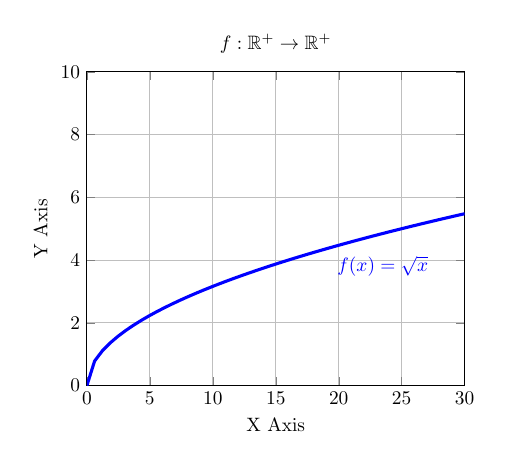
\begin{tikzpicture}[scale=0.7]
			\begin{axis}[
					xmax=30,
					xmin=0,
					ymax=10,
					ymin=0,
					samples=50,
					grid=major,
					xlabel={X Axis},
					ylabel={Y Axis},
					title={$f:\mathbb{R}^+\to\mathbb{R}^+$}
				]
				\addplot[blue, ultra thick,domain=0:30]{sqrt(x)} node[anchor=north west,pos=0.65] {$f(x)=\sqrt{x}$};
			\end{axis}
		\end{tikzpicture}
		\caption{The square root function only operates with positive numbers}
		\label{sketch:rem-sqrt-function}
	\end{figure}
	So, while it is sometimes convenient to follow the convention in \pref{equation}{eq-sqrt-abs-function},
	strictly speaking the square root function only ever takes on positive values
	(\textit{cf.} \pref{figure}{sketch:rem-sqrt-function}).
\end{rem}

\begin{definition}\label{def-floor-function}
	The floor function is defined by
	\begin{equation}
		\ffloor(x)=\floor{x}\defines\max\left\{m\in\mathbb{Z}\setbuild m\leq x\right\}
	\end{equation}
\end{definition}

\begin{definition}\label{def-ceiling-function}
	The ceiling function is defined by
	\begin{equation}
		\fceil(x)=\ceil{x}\defines\min\left\{n\in\mathbb{Z}\setbuild n\geq x\right\}
	\end{equation}
\end{definition}

\begin{definition}\label{def-dirichlet-function}
	The Dirichlet function is defined by
	\begin{equation}
		D(x)=\begin{cases}
			1\text{ if }x\in\mathbb{Q} \\
			0\text{ else }
		\end{cases}
	\end{equation}
\end{definition}

\begin{definition}\label{def-absolute-value-function}
	The absolute value function is defined by
	\begin{equation}
		\forall x\in\mathbb{R}: \abs{x}\defines\max\{x,-x\}=\begin{cases}
			x\text{ if } x \geq 0 \\
			-x \text{ else }
		\end{cases}
	\end{equation}
\end{definition}

\begin{thm}\label{thm-absolute-value-properties}
	Below are listed some of the properties related to the absolute value; for
	any $x\in\mathbb{R}$ the following holds:
	\begin{enumerate}
		\item $\abs{x} \geq 0$
		\item $\abs{x} \geq \pm x$
		\item $\abs{x} = \abs{-x}$
		\item $\abs{x} = 0 \iff x = 0$
		\item $\abs{xy} = \abs{x}\abs{y}$
		\item $\abs{x} + \abs{y} \geq \abs{x+y}$
		\item $\abs{x-y} \geq \abs[\big]{\abs{x}-\abs{y}}$
		\item $\abs{x} < M \iff -M < x < M$
	\end{enumerate}
\end{thm}

\begin{proof}
	Of theorem (\ref{thm-absolute-value-properties}).
	\begin{flushleft}
		In this proof we will only show property 6 of this theorem which is also
		known as the triangle inequality. From property 2 it follows that the sum
		of $\abs{x}\geq x$ and $\abs{y}\geq y$ equals
		\begin{equation}\label{tmp-absolute-value-properties:1}
			\abs{x} + \abs{y} \geq x + y
		\end{equation}
		Likewise, from $\abs{x}\geq -x$ and $\abs{y}\geq -y$ it follows that
		\begin{equation}\label{tmp-absolute-value-properties:2}
			\abs{x} + \abs{y} \geq -(x+y)
		\end{equation}
		Thus, by definition (\ref{def-absolute-value-function}) and equation
		(\ref{tmp-absolute-value-properties:1}) and (\ref{tmp-absolute-value-properties:2})
		we can conclude that
		\begin{equation*}
			\abs{x} + \abs{y} \geq \abs{x+y}
		\end{equation*}
	\end{flushleft}
\end{proof}

\begin{rem}
	A geometric interpretation of the absolute value function $\abs{x}$ is the
	distance from $x$ to $0$. Similarly, the absolute value of the difference
	$\abs{x-y}$ can be interpreted as the distance between $x$ and $y$. See also
	\hyperref[subsec-metric-spaces]{the subsection for metric spaces} for more
	more information on distances.
\end{rem}


\subsection{Limit Prerequisites}\label{subsec-limit-prerequisites}

\begin{definition}\label{def-interval-notation}
    As opposed to closed intervals, open and half-open intervals contain infinitely
    many elements. The $\infty$ symbol always needs to be paired with a parenthesis
    rather than a bracket because it is technically incorrect to think of infinity
    as a number. So far, we haven't agreed on a formal definition for the concept
    of infinity, but it will become important later when we discuss limits in more
    detail.
    \begin{enumerate}
        \item $(a,b)\defines\left\{x\setbuild a < x < b\right\}       \quad \text{(Open interval)}$
        \item $(a,b]\defines\left\{x\setbuild a < x \leq b\right\}    \quad \text{(Half-open interval)}$
        \item $[a,b)\defines\left\{x\setbuild a \leq x < b\right\}    \quad \text{(Half-closed interval)}$
        \item $[a,b]\defines\left\{x\setbuild a \leq x \leq b\right\} \quad \text{(Closed interval)}$
    \end{enumerate}
\end{definition}

\begin{definition}\label{def-epsilon-neighborhood}
    Let $a\in\mathbb{R}$ and $\varepsilon > 0$. Then the open interval 
    $(a-\varepsilon,a+\varepsilon)$ is called the epsilon neighborhood of $a$
    and is denoted by
    \begin{equation}
        \mathcal{U}_\varepsilon(a)\defines
        \left\{x \setbuild x\in\mathbb{R},\abs{x-a}<\varepsilon \right\}=
        (a-\varepsilon,a+\varepsilon)
    \end{equation}
\end{definition}

\begin{rem}\label{rem-epsilon-neighborhood}
    In reference to property 8 of theorem (\ref{thm-absolute-value-properties})
    we can note that
    \begin{equation}
        x\in(a-\varepsilon,a+\varepsilon) \iff \abs{x-a} < \varepsilon
    \end{equation}
\end{rem}

\begin{definition}\label{def-epsilon-punctured-neighborhood}
    Let $a\in\mathbb{R}$. For $\varepsilon>0$ we define the punctured epsilon 
    neighborhood of $a$, denoted by 
    \begin{equation}
        \mathcal{U}_{\varepsilon}^{\bolddot}(a)\defines
        \left\{x \setbuild x\in\mathbb{R}, 0<\abs{x-a}<\varepsilon\right\}=
        (a-\varepsilon,a+\varepsilon)\setminus\{a\}
    \end{equation}
\end{definition}

\begin{definition}\label{def-limit-point}
    Let $M\subset\mathbb{R}$ and $a\in\mathbb{R}$. Then, $a$ is called a limit 
    point\footnote{Or cluster point} of $M$ \textit{iff}
    \begin{equation}
        \bigwedge_{\varepsilon>0}(M\cap\mathcal{U}_\varepsilon^{\bolddot}\neq\emptyset)
    \end{equation}
\end{definition}

\begin{definition}\label{def-isolated-point}
    In contrast to definition (\ref{def-limit-point}), we call $a$ an isolated point
    of $M$ \textit{iff}
    \begin{equation}
        \neg\bigwedge_{\varepsilon>0}(M\cap\mathcal{U}_\varepsilon^{\bolddot}\neq\emptyset)
        \iff
        \bigvee_{\varepsilon>0}(M\cap\mathcal{U}_\varepsilon^{\bolddot}=\emptyset)
    \end{equation}
    \textit{i.e.} $a\in M\subset\mathbb{R}$ and $a$ is not a limit point.
\end{definition}

\begin{rem}
    If $a$ is an isolated point of $M$, then \cite[p.67]{wuest2009}
    \begin{align*}
        a\in M:\mathcal{U}_\varepsilon(a)
        &=(\{a\}\cup\mathcal{U}_\varepsilon^{\bolddot})\cap M \\
        &=(\{a\}\cap M)\cup(\mathcal{U}_\varepsilon^{\bolddot}\cap M) \\
        &=\{a\}
    \end{align*}
    Therefore, in the neighborhood of $a$ are no other elements of the set $M$.
\end{rem}

\begin{exm}\label{exm-limit-points}
    Find the set of all limit points for
    \begin{enumerate}
        \item $A\defines\displaystyle\bigcup_{n\in\mathbb{N}}\left(\frac{1}{n},2-\frac{1}{n}\right)$
        \item $B\defines\left\{x\in\mathbb{R}\setbuild x=n+\frac{1}{m}\quad\text{($n,m$ appropriate)}\right\}$
    \end{enumerate}
    \begin{flushleft}
        \textbf{\nth{1} Answer:} TODO
    \end{flushleft}
    \begin{flushleft}
        \textbf{\nth{2} Answer:} TODO
    \end{flushleft}
\end{exm}

\begin{definition}\label{def-bounded-sets}
    Let $A \subseteq\mathbb{R}$ be a set.
    \begin{enumerate}
        \item Then $A$ is called bounded from above if there exists $M\in\mathbb{R}$ 
        such that $x\leq M$ for any $x\in A$.
        \item Similarly, $A$ is bounded from below if there exists $m\in\mathbb{R}$ 
        such that $x\geq M$ for any $x\in A$.
        \item Finally, $A$ is called bounded if it is bounded from above and below.
        \footnote{Notice that the boundary points in this definition
        lay no claim to uniqueness.}
    \end{enumerate}
\end{definition}

\begin{exm}\label{exm-bounded-sets:1}
    \hfill
    \begin{enumerate}
        \item Consider the set of natural numbers: $\mathbb{N}$ is not bounded from above, but 
        below, \textit{i.e.} $1$ is a lower bound of $\mathbb{N}$.
        \item Let $A=(-3,2]$. Then this set is bounded from above and below.
        \item Let $B=\left\{\frac{1}{n}\setbuild n\in\mathbb{N}\right\}$. Then this
        set is bounded from above by $1$, and bounded from below by $0$.
    \end{enumerate}
\end{exm}

\begin{definition}\label{def-supremum-infimum-sets}
    Let $A\subset\mathbb{R}$ be a set.
    \begin{enumerate}
        \item $S$ is called the supremum of $A$ if it is the smallest upper bound 
        of $A$, and is denoted by $S=\sup(A)$.
        \item $I$ is called the infimum of $A$ if it is the largest lower bound 
        of $A$, and is denoted by $I=\inf(A)$.
    \end{enumerate}
\end{definition}

\begin{exm}\label{exm-bounded-sets:2}
    Consider the sets from \pref{example}{exm-bounded-sets:1}. Then\footnote{Remark:
    $\mathbb{N}\defines\{1,2,3,\dots\}$}
    \begin{enumerate}
        \item $\inf(\mathbb{N})=1$
        \item $\inf(A)=-3$ and $\sup(A)=2$
        \item $\inf(B)=0$ and $\sup(B)=1$
    \end{enumerate}
\end{exm}

\begin{definition}\label{def-maximum-minimum}
    Let $A\subset\mathbb{R}$ be a set.
    \begin{enumerate}
        \item If $S=\sup(A)$, then $S\in A$ is also a maximum of $A$ and is denoted by $S=\max(A)$.
        \item If $I=\inf(A)$, then $I\in A$ is also a minimum of $A$ and is denoted by $I=\min(A)$.
    \end{enumerate}
\end{definition}

\begin{exm}\label{exm-bounded-sets:3}
    Expanding on the results from example (\ref{exm-bounded-sets:2}), we note that
    \begin{enumerate}
        \item $\min(\mathbb{N})=1$
        \item $\min(A)=\text{\gls{dne}}$ and $\max(A)=2$
        \item $\min(B)=\text{\gls{dne}}$ and $\max(B)=1$
    \end{enumerate}
\end{exm}


\subsection{Limits}\label{subsec-limits}

\begin{definition}\label{def-epsilon-delta-definition-limit}
    Let $f(x)$ be a function with $a,b\in\mathbb{R}$ with $a$ as a limit point of $\domain{f}$.
    Then the the function $f$ has the limit $b$ as $x$ approaches $a$, \textit{i.e.}    
    \begin{equation}
        \bigwedge_{\varepsilon>0}\bigvee_{\delta>0}\bigwedge_{x\in\domain{f}} 
        \left(0<\abs{x-a}<\delta\implies\abs{f(x)-b}<\varepsilon\right)
    \end{equation}
    The limit of this function is denoted by
    \begin{equation}
        \lim_{x\to a}f(x)=b,
    \end{equation}
\end{definition}

\begin{rem}
    The equation $\displaystyle\lim_{x\to a}f(x)=b$ is equivalent to the following
    expressions:
    \begin{enumerate}
        \item For $f$ there exists a limit (point) at $a$.
        \item This limit of $f$ is equal to $b$.
    \end{enumerate}
    In other words, $f$ has a limit at $a$ if
    \begin{equation*}
        \bigvee_{b\in\mathbb{R}}\bigwedge_{\varepsilon>0}\bigvee_{\delta>0}\bigwedge_{x\in\domain{f}} 
        \left(0<\abs{x-a}<\delta \implies \abs{f(x)-b}<\varepsilon\right)
    \end{equation*}
\end{rem}

\begin{exm}\label{exm-epsilon-delta-definition-limit:1}
    Show that 
    \begin{equation*}
        \lim_{x\to3}\frac{x-1}{2}=1
    \end{equation*}
    by using the epsilon-delta definition for limits.
    \begin{flushleft}
        \textbf{Answer}: Let $\varepsilon>0$ and $b\in\mathbb{R}$. Take 
        $\delta\defines2\varepsilon$; Then $\abs{x-3}<\delta$, which implies
        \begin{align*}
            \abs{f(x)-b}&=\abs[\Bigg]{\frac{x-1}{2}-1}\\
                        &=\frac{\abs{x-3}}{2}\\
                        &<\frac{\delta}{2}\\
                        &=\varepsilon
        \end{align*}
    \end{flushleft}
\end{exm}

\begin{exm}\label{exm-epsilon-delta-definition-limit:2}
    Show that for some $a\in\mathbb{R}$,
    \begin{equation*}
        \lim_{x\to a}\sin(x)=\sin(a)
    \end{equation*}
    by using the epsilon-delta definition for limits.
    \begin{flushleft}
        \textbf{Answer}: Let $\varepsilon>0$ and $b\in\mathbb{R}$. Take 
        $\varepsilon\defines\delta$ such that $\abs{x-a}<\delta$. Further, recall that
        \begin{align*}
            &\text{(A)}:\forall\alpha\in\mathbb{R}:\abs{\cos(\alpha)}\leq1\\
            &\text{(B)}:\forall\alpha\in\mathbb{R}:\abs{\sin(\alpha)}\leq\abs{\alpha}
        \end{align*}
        \begin{align*}
            \abs{f(x)-b}&=\abs{\sin(x)-\sin(a)}\\
                        &=\abs[\Bigg]{2\sin\left(\frac{x-a}{2}\right)\cos\left(\frac{x+a}{2}\right)}\\
                        &=2\cdot\abs[\Bigg]{\sin\left(\frac{x-a}{2}\right)}\abs[\Bigg]{\cos\left(\frac{x+a}{2}\right)}\\
                        &\leq 2\cdot\frac{\abs{x-a}}{2} && \text{note (A) \& (B)}\\
                        &=\varepsilon
        \end{align*}
    \end{flushleft}
\end{exm}

\begin{exm}\label{exm-epsilon-delta-definition-limit:3}
    Show \cite[p.69]{wuest2009} that the function $f(x)=\tfrac{x^2-3x+2}{x(x-1)}$
    with $x\in\mathbb{R}\setminus\{0,1\}$ has the limit $b=-1$ as $x\to1$.
    \begin{flushleft}
        \textbf{Answer}: Let $\varepsilon>0$.
        \begin{align}
            \abs{f(x)-(-1)}&=\abs[\Bigg]{\frac{x^2-3x+2}{x(x-1)}+1}\nonumber\\
                           &=\abs[\Bigg]{\frac{(x-2)(x-1)}{x(x-1)}+1}\nonumber\\
                           &=\abs[\Bigg]{\frac{x-2}{x}+1}\nonumber\\
                           &=\abs[\Bigg]{\frac{2x-2}{x}}\nonumber\\
                           &=\frac{2}{\abs{x}}\cdot\abs{x-1}\label{eq3-epsilon-delta-definition-limit:1}
        \end{align}
        Since we aim for the neighborhood of $x=1$ we can impose the following
        restriction on this inequality:
        \begin{equation}\label{eq3-epsilon-delta-definition-limit:2}
            0<\abs{x-1}<\frac{1}{2}
        \end{equation}
        This in turn implies
        \begin{align}
            \abs{x}&=\abs{x-1+1}\nonumber\\
                   &\geq1-\abs{x-1}\nonumber\\
                   &>1-\frac{1}{2} && \text{\pref{equation}{eq3-epsilon-delta-definition-limit:2}}\nonumber\\
                   &=\frac{1}{2}\label{eq3-epsilon-delta-definition-limit:3}
        \end{align}
        Hence,
        \begin{align}
            \abs{f(x)-b}&=\frac{2}{\abs{x}}\cdot\abs{x-1} && \text{\pref{equation}{eq3-epsilon-delta-definition-limit:1}}\nonumber\\
                        &<\frac{2}{\tfrac{1}{2}}\cdot\abs{x-1} && \text{\pref{equation}{eq3-epsilon-delta-definition-limit:3}}\nonumber\\
                        &=4\cdot\abs{x-1}\label{eq3-epsilon-delta-definition-limit:4}
        \end{align}
    \end{flushleft}
    Let $q(\varepsilon)\defines\min\left\{\tfrac{\varepsilon}{4},\tfrac{1}{2}\right\}$.
    Then for all $\varepsilon>0$ there exists a $\delta\defines q(\varepsilon)$ such that
    for $x\in\domain{f}$ it follows that
    \begin{align*}
        0<\abs{x-1}<\delta \implies \abs{f(x)-(-1)}&<4\cdot\abs{x-1}&&\text{\pref{equation}{eq3-epsilon-delta-definition-limit:4}}\\
                                                   &<4\cdot\frac{\varepsilon}{4}\\
                                                   &=\varepsilon
    \end{align*}
\end{exm}

\begin{exm}\label{exm-epsilon-delta-definition-limit:4}
    Show that the function $f(x)=\tfrac{x^2-4x+3}{2x-6}$ with $x\in\mathbb{R}\setminus\{3\}$
    has the limit $b=1$ as $x\to3$.
    \begin{flushleft}
        \textbf{Answer}: Let $\varepsilon>0$. Define $\delta\defines2\varepsilon$,
        such that $\abs{x-3}<\delta$, wherefore
        \begin{align*}
            \abs{f(x)-b}&=\abs[\Bigg]{\frac{x^2-4x+3}{2x-6}-1}\\
                        &=\abs[\Bigg]{\frac{(x-1)(x-3)}{2(x-3)}-1}\\
                        &=\abs[\Bigg]{\frac{1}{2}(x-1)-1}\\
                        &=\abs[\Bigg]{\frac{1}{2}x-\frac{3}{2}}\\
                        &=\frac{1}{2}\abs{x-3}\\
                        &<\frac{1}{2}\cdot2\varepsilon\\
                        &=\varepsilon
        \end{align*}
    \end{flushleft}
\end{exm}

\begin{exm}\label{exm-epsilon-delta-definition-limit:5}
    Show that for $a>0$ ($a\in\mathbb{R}$),
    \begin{equation*}
        \sqrt{x}\tolim{x}{a}\sqrt{a}
    \end{equation*}
    \begin{flushleft}
        \textbf{Answer}: Let $\varepsilon>0$. When we define $\delta\defines\min\left\{a,\varepsilon\sqrt{a}\right\}$,
        then $\abs{x-a}<\delta$ implies that
        \begin{align*}
            \abs{f(x)-b}&=\abs[\big]{\sqrt{x}-\sqrt{a}}\\
                        &=\frac{\abs[\big]{\sqrt{x}-\sqrt{a}}\left(\sqrt{x}+\sqrt{a}\right)}{\sqrt{x}+\sqrt{a}}\\
                        &=\frac{\abs{x-a}}{\sqrt{x}+\sqrt{a}}\\
                        &<\frac{\abs{x-a}}{\sqrt{a}}\\
                        &<\frac{\varepsilon\sqrt{a}}{\sqrt{a}}\\
                        &=\varepsilon
        \end{align*}
        Therefore,
        \begin{equation*}
            \lim_{x\to a}\sqrt{x}=\sqrt{a}
        \end{equation*}
    \end{flushleft}
\end{exm}

\begin{rem}\label{rem-undefined-limits}
    Examples of functions where \pref{definition}{def-epsilon-delta-definition-limit} breaks:
    \begin{enumerate}
        \item For any $a\in\mathbb{Z}$, the limit of $f(x)=\floor{x}$ does not exists.
        \item The limit $\displaystyle\lim_{x\to0}\tfrac{1}{x}$ does not exists.
        \item The limit $\displaystyle\lim_{x\to0}\tfrac{1}{x^2}$ does not exists.
        \item The limit $\displaystyle\lim_{x\to0}\sin\left(\tfrac{1}{x}\right)$ does not exists.
    \end{enumerate}
\end{rem}

\begin{thm}\label{thm-limit-arithmetic}
    Let $\displaystyle\lim_{x \to a}f(x) = b_1$ and $\displaystyle\lim_{x \to a}g(x) = b_2$
    be two well-defined limits. Then the following statements hold:
    \begin{enumerate}
        \item $c \cdot f(x) \tolim{x}{a} c \cdot b_1 \quad (c\in\mathbb{R})$
        \item $f(x) + g(x) \tolim{x}{a} b_1 + b_2$
        \item $f(x) \cdot g(c) \tolim{x}{a} b_1 \cdot b_2$
        \item $\tfrac{f(x)}{g(x)} \tolim{x}{a} \tfrac{b_1}{b_2} \quad (b_2 \neq 0)$
    \end{enumerate}
\end{thm}


\begin{proof}
    Of \pref{theorem}{thm-limit-arithmetic}.
    \begin{flushleft}
        \textbf{\nth{2} Property}. From \pref{definition}{def-epsilon-delta-definition-limit}
        we can note that
        \begin{align*}
            &\forall\varepsilon>0\;\exists\delta_1>0:\,\abs{x-a}<\delta_1\implies\abs{f(x)-b_1}<\frac{\varepsilon}{2}\\
            &\forall\varepsilon>0\;\exists\delta_2>0:\,\abs{x-a}<\delta_2\implies\abs{g(x)-b_2}<\frac{\varepsilon}{2}
        \end{align*}        
        Define $\delta\defines\min\{\delta_1,\delta_2\}$ Then, if $\abs{x-a}<\delta$,
        it follows from the triangle inequality that
        \begin{align*}
            \abs{f(x)+g(x)-(b_1+b_2)}&=\abs{(f(x)-b_1)+(g(x)-b_2)}\\
                                     &\leq\abs{f(x)-b_1}+\abs{g(x)-b_2}\\
                                     &<\frac{\varepsilon}{2}+\frac{\varepsilon}{2}\\
                                     &=\varepsilon
        \end{align*}
    \end{flushleft}
\end{proof}

\begin{exm}
    Find the limit of
    \begin{equation*}
        \lim_{x \to 0}\left(\arctan\left(2\sqrt{\frac{\cos(x)}{3x+4}}\right)\right)=\frac{\pi}{4}
    \end{equation*}
    \begin{flushleft}
        \textbf{Answer}: TODO
    \end{flushleft}
\end{exm}

\begin{thm}\label{thm-absolute-value-of-limit:1}
    If $f(x) \tolim{x}{a} 0$, then this is equivalent to
    $\abs{f(x)} \tolim{x}{a} 0$.
\end{thm}

\begin{thm}\label{thm-absolute-value-of-limit:2}
    Let $b\in\mathbb{R}$. If $f(x) \tolim{x}{a} b$, then 
    this implies $\abs{f(x)} \tolim{x}{a} \abs{b}$.
\end{thm}

\begin{rem}
    Note that the opposite direction of \pref{theorem}{thm-absolute-value-of-limit:2}
    is in general not true. A counter example for this would be the 
    \hyperref[def-dirichlet-function]{Dirichlet function}.
\end{rem}

\begin{proof}
    Of \pref{theorem}{thm-absolute-value-of-limit:2}.
    \begin{flushleft}
        Let $\varepsilon>0$. Then $\abs{x-a}<\delta$ implies that
        \begin{align*}
            \abs[\big]{\abs{f(x) - \abs{b}}} &\leq \abs{f(x) - b} \\
                                             &<\varepsilon
        \end{align*}
        by using the reverse triangle inequality for absolute values.
    \end{flushleft}
\end{proof}

\begin{thm}\label{thm-limit-monotonicity}
    Let $f(x) \geq g(x)$ for any $x\in\mathcal{U}_{\varepsilon}^{\bolddot}(a)$. 
    If the limit of $f(x)$ and $g(x)$ exist, then
    \begin{equation*}
        \lim_{x \to a}f(x) \geq \lim_{x \to a}g(x)
    \end{equation*}
\end{thm}

\begin{rem}
    As for \pref{theorem}{thm-limit-monotonicity}, if $f(x) \geq 0$,
    then
    \begin{equation*}
        \lim_{x \to a}f(x) \geq 0
    \end{equation*}
\end{rem}

\begin{rem}
    \pref{Theorem}{thm-limit-monotonicity} does not hold if we replace the greater
    than or equal to inequality with a strictly greater than inequality.
\end{rem}

\begin{thm}\label{thm-unique-limit}
    If the limit of $\displaystyle\lim_{x\to a}f(x)=b\in\mathbb{R}$ exists, then $b$ is unique.
\end{thm}

\begin{proof}
    Of \pref{theorem}{thm-unique-limit}.
    \begin{flushleft}
        Assume \gls{wlog} that $b<c$ are both limits of this function. Define
        $\varepsilon\defines\tfrac{c-b}{3}>0$. Then by 
        \pref{definition}{def-epsilon-delta-definition-limit} we have that
        \begin{equation}\label{eq-unique-limit:1}
            \exists\delta_1\text{ s.t. }a-\delta_1<x<a+\delta_1 \implies b-\varepsilon<f(x)<b+\varepsilon
        \end{equation}
        Likewise we know that
        \begin{equation}\label{eq-unique-limit:2}
            \exists\delta_2\text{ s.t. }a-\delta_1<x<a+\delta_1 \implies c-\varepsilon<f(x)<c+\varepsilon
        \end{equation}
    \end{flushleft}
    Therefore by \pref{equation}{eq-unique-limit:1} and \pref{equation}{eq-unique-limit:2},
    it follows that
    \begin{equation*}
        \left(f(x)<b+\varepsilon<c+\varepsilon\right)\land\left(c+\varepsilon<f(x)\right)
    \end{equation*}
    which is a contradiction. 
\end{proof}

\begin{thm}\label{def-limit-is-bounded}
    If the limit of $\displaystyle\lim_{x\to a}f(x)=b\in\mathbb{R}$ exists, then
    $f$ is bounded in a neighborhood of $a$.
\end{thm}

\begin{thm}\label{thm-sandwich-theorem}
    Suppose that for any $x$ in a neighborhood of $a$
    \begin{equation*}
        h(x) \leq f(x) \leq g(x)
    \end{equation*}
    Further assume that
    \begin{equation*}
        \lim_{x \to a}h(x) = b = \lim_{x \to a}g(x)
    \end{equation*} 
    Then it follows that
    \begin{equation*}
        \lim_{x \to a}f(x) = b
    \end{equation*}
\end{thm}

\begin{proof}
    Of \pref{theorem}{thm-sandwich-theorem}.
    \begin{flushleft}
        Let $\varepsilon>0$. Take $\delta\defines\min\{\delta_1,\delta_2\}$ where
        \begin{align*}
            &0 < \abs{x - a} < \delta_1 \implies \abs{g(x) - b} < \varepsilon \iff b - \varepsilon < g(x) < b + \varepsilon, \\
            &0 < \abs{x - a} < \delta_2 \implies \abs{h(x) - b} < \varepsilon \iff b - \varepsilon < h(x) < b + \varepsilon
        \end{align*}
        Therefore, if $0 < \abs{x - a} < \delta$,
        \begin{equation*}
            b - \varepsilon < h(x) \leq f(x) \leq g(x) < b + \varepsilon
        \end{equation*}
        which is equivalent to
        \begin{equation*}
            \abs{f(x) - b} < \varepsilon \iff \lim_{x \to a}f(x) = b
        \end{equation*}
    \end{flushleft}
\end{proof}

\begin{thm}\label{thm-product-of-bounded-zero-limit}
    If $\displaystyle\lim_{x \to a}f(x) = 0$ and $g(x)$ is bounded in a neighborhood
    of $a$, then
    \begin{equation*}
        \lim_{x \to a} \left(f(x)\cdot g(x)\right) = 0
    \end{equation*}
\end{thm}

\begin{proof}
    Of \pref{theorem}{thm-product-of-bounded-zero-limit}.
    \begin{flushleft}
        Since $g(x)$ is bounded, we can write $\abs{g(x)} \leq M$. So,
        \begin{align*}
            &-M \leq \abs{g(x)} \leq M\\
            \implies
            &-M\cdot\abs{f(x)} \leq \abs{f(x)}\cdot\abs{g(x)} \leq M\cdot \abs{f(x)}\\
            \implies
            &-M\cdot \lim_{x \to a}\abs{f(x)} \leq  \lim_{x \to a}\left(\abs{f(x)}\cdot\abs{g(x)}\right) \leq M \cdot \lim_{x \to a}\abs{f(x)}\\
            \implies
            &-M \cdot 0 \leq \abs{f(x)}\cdot\abs{g(x)} \leq M \cdot 0 && \text{\pref{theorem}{thm-absolute-value-of-limit:1}} \\
            \implies
            & 0 \leq \abs{f(x)}\cdot\abs{g(x)} \leq 0 && \text{\pref{theorem}{thm-limit-arithmetic}}\\
            \implies
            &\lim_{x \to a}\left(\abs{f(x)}\cdot\abs{g(x)}\right)=0 && \text{\pref{theorem}{thm-sandwich-theorem}}\\
            \implies
            &\lim_{x \to a}\left(f(x)\cdot g(x)\right)=0 && \text{\pref{theorem}{thm-absolute-value-of-limit:1}} \\
        \end{align*}
    \end{flushleft}
\end{proof}

\begin{exm}
    The limit of the function 
    \begin{equation*}
        f(x) = x\cdot\sin\left(\frac{1}{x}\right)
    \end{equation*}
    as $x \to 0$ is
    \begin{equation*}
        \lim_{x \to 0}\left(x\cdot\sin\left(\frac{1}{x}\right)\right)=0
    \end{equation*}
    by \pref{theorem}{thm-product-of-bounded-zero-limit} since $\sin\left(\tfrac{1}{x}\right)$
    is bounded\footnote{But in and of itself not defined at $x=0$} by $[-1,1]$ 
    and the left factor of this function is $x=0$ as $x \to 0$.
\end{exm}

\begin{definition}\label{def-one-sided-limits}
    We denote the one-sided limit of the function $f(x)$ approached from the right by
    \begin{equation*}
        \lim_{x \to a^+}f(x)=b
    \end{equation*}
    if and only if
    \begin{equation}
        \forall\varepsilon>0\;\exists\delta>0:x\in(a,a+\delta)\implies\abs{f(x)-b}<\varepsilon
    \end{equation}
    Conversely, the left-sided limit is denoted by
    \begin{equation*}
        \lim_{x \to a^-}f(x)=b
    \end{equation*}
    if and only if
    \begin{equation}
        \forall\varepsilon>0\;\exists\delta>0:x\in(a-\delta,a)\implies\abs{f(x)-b}<\varepsilon
    \end{equation}
\end{definition}

\begin{rem}\label{rem-one-sided-limits}
    With respect to \pref{definition}{def-one-sided-limits}, note that there exist
    several equivalent notations. So, the right-sided limit of $f(x)$ can be denoted
    by
    \begin{equation*}
        \lim_{x \to a^+}f(x)=b
        \iff
        \lim_{x \underset{x>a}{\to} a}f(x)=b
        \iff
        \lim_{x\searrow  a}f(x)=b
    \end{equation*}
    Similarly, at times the left-sided limits may be denoted by
    \begin{equation*}
        \lim_{x \to a^-}f(x)=b
        \iff
        \lim_{x \underset{x<a}{\to} a}f(x)=b
        \iff
        \lim_{x \nearrow a}f(x)=b
    \end{equation*}
\end{rem}

\begin{thm}\label{thm-limit-exists-one-sided-limits}
    The limit of $f(x) \to b$ exists as $x \to a$ if and only if the left-sided
    limit as well as the right-sided limit of $f$ exists with
    \begin{equation}
        \lim_{x \to a}f(x)=b \iff \lim_{x \to a^+}f(x)=b=\lim_{x \to a^-}f(x)
    \end{equation}
\end{thm}

\begin{proof}
    Of \pref{theorem}{thm-limit-exists-one-sided-limits}.
    \begin{flushleft}
        TODO
    \end{flushleft}
\end{proof}

\begin{exm}\label{exm-important-sin-over-x-limit}
    Show that\footnote{This is a very useful limit that we are going to encounter
    more often in the near future.}
    \begin{equation}\label{eq-important-sin-over-x-limit}
        \lim_{x \to 0}\frac{\sin(x)}{x}=1
    \end{equation}
    \begin{flushleft}
        \textbf{Answer}: From figure (??) we can derive two observations:
        \begin{equation*}
            \forall x\in\left(0,\frac{\pi}{2}\right)\implies \sin(x)<x
        \end{equation*}
        Notice also that
        \begin{equation*}
            x < \tan(x)
        \end{equation*}
        So, this implies
        \begin{equation}\label{eq-important-sin-over-x-limit:1}
            \sin(x) < x < \tan(x)
        \end{equation}
        Furthermore, figure (??) reveals that
        \begin{equation*}
            \forall x\in\mathbb{R}:\abs{\sin(x)}\leq\abs{x}
        \end{equation*}
        From \pref{equation}{eq-important-sin-over-x-limit:1} follows that for all
        $\tfrac{\pi}{2}>x>0$:
        \begin{align*}
            \implies 
            &\frac{1}{\sin(x)} > \frac{1}{x} > \frac{1}{\tan(x)} \\
            \implies 
            &1 > \frac{\sin(x)}{x} > \cos(x) \\
            \implies 
            &1 > \lim_{x \to 0^+}\frac{\sin(x)}{x} > \lim_{x \to 0^+}\cos(x) \\
            \implies
            &1 > \lim_{x \to 0^+}\frac{\sin(x)}{x} > 1\\
            \implies 
            &\lim_{x \to 0^+}\frac{\sin(x)}{x}=1 && \text{theorem (\ref{thm-sandwich-theorem})}
        \end{align*}
        A similar argument can be made for 
        \begin{align*}
            \forall x\in\left(-\frac{\pi}{2},0\right):\lim_{x \to 0^-}\frac{\sin(x)}{x}=1
        \end{align*}
        Last but not least, \pref{theorem}{thm-limit-exists-one-sided-limits} ensures
        that the limit in \pref{equation}{eq-important-sin-over-x-limit} exists.
    \end{flushleft}
\end{exm}

\begin{thm}\label{thm-monotone-one-sided-limits}
    Assume that $f$ is monotone on some interval $[a,b]$. Then $f$ has one-sided
    limits at every point.
\end{thm}

\begin{definition}\label{def-infinity-limits}
    Let $f$ be a function such that\footnote{In other words, $\infty$ is a limit
    point of the domain of $f$}
    \begin{equation}
        \forall c\in\mathbb{R}: (c,\infty)\cap\domain{f}\neq\emptyset
    \end{equation}
    Next let $b\in\mathbb{R}$. We say that $f(x) \to b$ for $x \to \infty$ if and only if
    \footnote{Similarly, we can define the limit for $f(x) \to b$ as $x \to -\infty$}
    \begin{equation}
        \bigwedge_{\varepsilon>0}\bigvee_{c\in\mathbb{R}}\bigwedge_{x\in\domain{f}}
        \left(x>c \implies \abs{f(x) - b}<\varepsilon\right)
    \end{equation}
    Then this is equivalent to \cite[p.70]{wuest2009}
    \begin{equation}
        \lim_{x \to \infty}f(x)=b
    \end{equation}
\end{definition}

\begin{rem}
    Definition (\ref{def-infinity-limits}) works with all previously encountered theorems.
\end{rem}

\begin{exm}\label{exm-infinity-limit:1}
    Let $f$ be defined by \cite[p.71]{wuest2009}
    \begin{equation*}
        f(x)\defines\frac{3x^2-2x+1}{x^2+5x}
    \end{equation*}
    where $x\in(0,\infty)$. Show that
    \begin{equation*}
        \lim_{x \to \infty}f(x)=3
    \end{equation*} 
    \begin{flushleft}
        \textbf{Answer}: First observe, that for very large $x$ the quadratic terms
        in the numerator and denominator dominate over the other terms in the long
        run. Keeping this in mind we can make an intelligent guess for the limit point
        $f(x) \to 3$ as $x \to \infty$. Now for the formal part of this proof: Let $x>0$.
        Then, for $a(\varepsilon)\defines\max\left\{1,\tfrac{18}{\varepsilon}\right\}$ it
        follows that
        \begin{align*}
            \abs{f(x) - b} &= \abs[\Bigg]{\frac{3x^2-2x+1}{x^2+5x}-3}\\
                           &= \abs[\Bigg]{\frac{3x^2-2x+1-3x^2-15x}{x^2+5x}}\\
                           &= \abs[\Bigg]{\frac{-17x+1}{x^2+5x}}\\
                           &\leq {\frac{\abs{-17x}+\abs{1}}{x^2+5x}}\\
                           &= \frac{17x}{x^2+5x} + \frac{1}{x^2+5x}\\
                           &\leq \frac{17x}{x^2} + \frac{1}{x^2}\\
                           &\leq \frac{18}{x} && \text{if } x\geq1\\
                           &< \frac{18}{\tfrac{18}{\varepsilon}}\\
                           &= \varepsilon
        \end{align*}
        in other words for every $\varepsilon>0$ there exists a $c\in\mathbb{R}$
        such that $c\defines a(\varepsilon)$ for which is true that
        \begin{equation*}
            x>c \implies \abs{f(x)-b}<\varepsilon
        \end{equation*}
        which means that $f(x)$ converges towards $3$ as $x$ approaches infinity.
    \end{flushleft}
\end{exm}

\begin{definition}\label{def-infinite-limits}
    We say a function has an infinite limit at infinity when
    \begin{equation}
        \bigwedge_{c\in\mathbb{R}}\bigvee_{\delta>0}
        \left(\abs{x-a}<\delta \implies f(x)>c\right)
    \end{equation}
    which is denoted by
    \begin{equation}
        \lim_{x \to a}f(x)=\infty
    \end{equation}
    Another frequently used expression to describes this behavior is divergence;
    limits that exhibit this type behavior are said to diverge. 
\end{definition}

\begin{exm}\label{exm-infinity-limit:3}
    Use \pref{definition}{def-infinite-limits} to show that
    \begin{equation}
        \lim_{x \to 0}\frac{1}{x^2}=\infty
    \end{equation}
    \begin{flushleft}
        \textbf{Answer}: Let $c\in\mathbb{R}^+$ such that $\delta\defines\tfrac{1}{\sqrt{c}}$.
        Then, it follows that
        \begin{equation*}
            0<\abs{x-0}<\delta \implies \abs{x} < \frac{1}{\sqrt{c}} \implies \frac{1}{x^2} > c
        \end{equation*}
    \end{flushleft}
\end{exm}

\begin{rem}
    Beware: for $f(x) \to \pm\infty$ not all theorems hold, in particular 
    \pref{theorem}{thm-limit-arithmetic} is only partially true.
\end{rem}

\begin{thm}\label{thm-pizza-theorem}
    If $g(x) \geq f(x)$ in a neighborhood of $a$ and $f(x) \to \infty$ as $x \to a$,
    then $g(x) \to \infty$ for $x \to a$.
\end{thm}


\subsection{Sequences}\label{subsec-sequences}

\begin{definition}\label{def-sequence}
	An infinite ordered set of real\footnote{This document restricts the definition
		to the set of real numbers, but in other courses it can be more abstract than that}
	numbers is called a sequence, most formally denoted by $\{a_n\}_{n=1}^\infty$,
	or just $a_n$.
\end{definition}

\begin{definition}\label{def-sequence-recursive:1}
	Let $a\in\mathbb{N}$. We define \cite[p.51]{wuest2009}
	\begin{align*}
		a_1     & = a + 1   \\
		a_{n+1} & = a_n + 1
	\end{align*}
\end{definition}

\begin{definition}\label{def-sequence-recursive:2}
	Let $a\in\mathbb{R}\setminus\{0\}$. We define \cite[p.51]{wuest2009}
	\begin{align*}
		a^0     & = 1                                                                         \\
		a^{n+1} & = a^n \cdot n &  & (n\in\mathbb{N}_0\defines\mathbb{N}\cup\{0\}=\mathbb{Z})
	\end{align*}
\end{definition}

\begin{definition}\label{def-sequence-recursive:3}
	Let $n\in\mathbb{N}_0$. We define \cite[p.51]{wuest2009}
	\begin{align*}
		0!     & = 1       \\
		(n+1)! & = n!(n+1)
	\end{align*}
	This is known as the faculty.
\end{definition}

\begin{definition}\label{def-sequence-recursive:4}
	Let $c\in\mathbb{Z}$ and $\{a_n\}_{n\in\mathbb{Z}_c}$ be sequences. We define \cite[p.51]{wuest2009}
	\begin{align*}
		\sum_{k=c}^n a_k     & = a_c                                                \\
		\sum_{k=c}^{n+1} a_k & = \sum_{k=c}^n a_k + a_{n+1} &  & (n\in\mathbb{Z}_c)
	\end{align*}
	This is known as the sum.
\end{definition}

\begin{definition}\label{def-sequence-recursive:5}
	Let $c\in\mathbb{Z}$ and $\{a_n\}_{n\in\mathbb{Z}_c}$ be sequences. We define \cite[p.51]{wuest2009}
	\begin{align*}
		\prod_{k=c}^n a_k     & = a_c                                                                  \\
		\prod_{k=c}^{n+1} a_k & = \left(\prod_{k=c}^n a_k\right) \cdot a_{n+1} &  & (n\in\mathbb{Z}_c)
	\end{align*}
	This is known as the product.
\end{definition}

\begin{rem}
	A sequence can also be written as a function $f:\mathbb{N}\to\mathbb{R}$,
	where $a_n = f(n)$.
\end{rem}

\begin{definition}\label{def-sequence-limit}
	Let $a_n$ be a sequence. We say that
	\begin{equation*}
		\lim_{n\to\infty}a_n=b
	\end{equation*}
	for $b\in\mathbb{R}$ if and only if
	\begin{equation*}
		\forall\varepsilon>0\;\exists N\in\mathbb{N}: n>N \implies \abs{a_n - b}<\varepsilon
	\end{equation*}
\end{definition}

\begin{rem}\label{rem-remarkable-sequences}
	What follows is a short list of some of the more notable sequences that we will
	get to know over time:
	\begin{enumerate}
		\item Linear sequence: $a_n=n$, \textit{e.g.} $1,3,4,5,\dots$
		\item Harmonic sequence: $a_n=\tfrac{1}{n}$, \textit{e.g.} $1,\tfrac{1}{2},\tfrac{1}{3},\tfrac{1}{4},\tfrac{1}{5},\dots$
		\item Alternating sequence: $a_n=(-1)^n$, \textit{e.g.} $-1,1,-1,1,-1,\dots$
		\item Alternating harmonic sequence: $a_n=\tfrac{(1)^{n}}{n}$, \textit{e.g.} $1,-\tfrac{1}{2},\tfrac{1}{3},-\tfrac{1}{4},\tfrac{1}{5},\dots$
		\item Arithmetic sequence: $a_n=5+2(n-1)$, \textit{e.g.} $5,7,9,11,13,\dots$
		\item Geometric sequence: $a_n=3\cdot2^{n-1}$, \textit{e.g.} $3,6,12,24,48,\dots$
		\item Constant sequence: $a_n=2$, \textit{e.g.} $2,2,2,2,2,\dots$
		\item Case sequence: $a_n=\begin{cases}1\text{ if }n\text{ is even}\\n\text{ else}\end{cases}$, \textit{e.g.} $1,1,3,1,5,\dots$
		\item Sequence of prime numbers\footnote{To date there exists no known formula for this sequence}, \textit{e.g.} $2,3,5,7,11,\dots$
		\item Sequence of digital digits of $\pi$, \textit{e.g.} $1,4,1,5,9,\dots$
		\item Recursive sequence: $a_n=\begin{cases}a_1=2\\a_n=3a_{n-1}^2\end{cases}$, \textit{e.g.} $2,12,432,559.872,\dots$
	\end{enumerate}
\end{rem}

\begin{exm}\label{exm-harmonic-sequence}
	Let $a_n$ be the harmonic sequence. Show that $\tfrac{1}{n}\to0$ as $n\to\infty$.
	\begin{flushleft}
		\textbf{Answer}: Let $\varepsilon>0$ and $N>\tfrac{1}{\varepsilon}$. Then,
		\begin{align*}
			\abs{f(x) - b} & = \abs[\Bigg]{\frac{1}{n}-0} \\
			               & = \frac{1}{n}                \\
			               & < \frac{1}{N}                \\
			               & < \varepsilon
		\end{align*}
	\end{flushleft}
\end{exm}

\begin{rem}
	Adding, dropping or changing any finite number of elements in a sequence does
	not affect the limit.
\end{rem}

\begin{thm}\label{thm-sequence-unique-limit}
	If $a_n$ has a limit, then the limit is unique.
\end{thm}

\begin{thm}\label{thm-sequence-limit-bounded}
	If $a_n$ has a limit, then $a_n$ is also bounded.
\end{thm}

\begin{rem}\label{rem-sequence-limit-bounded}
	\pref{Theorem}{thm-sequence-limit-bounded} only works in one direction; the
	limit might not exist if the sequence is bounded. Take for instance the alternating
	sequence as an counter example. Conversely, if the sequence is not bounded, then
	it has no finite limit.
\end{rem}

\begin{proof}
	Of \pref{theorem}{thm-sequence-limit-bounded}.
	\begin{flushleft}
		Suppose that $a_n$ has a limit, \textit{i.e.}
		\begin{equation*}
			\lim_{n\to\infty}a_n=b
		\end{equation*}
		then define
		\begin{equation*}
			M\defines\max\left\{b+1,a_1,a_2,\dots,a_N\right\}
		\end{equation*}
		for $n>N$ such that $a_n\in(b-1,b+1)$. We define
		\begin{equation*}
			m\defines\min\left\{b-1,a_1,a_2,\dots,a_N\right\}
		\end{equation*}
		Hence, $m \leq a_n \leq M$ for all $n\in\mathbb{N}$.
	\end{flushleft}
\end{proof}

\begin{thm}\label{thm-sequence-arithmetic}
	Let $a_n \seqinfty{n} L$ and $b_n \seqinfty{n} K$ be two limited sequences. Then
	\begin{enumerate}
		\item $\forall c\in\mathbb{R}:c \cdot a_n \seqinfty{n} c \cdot L$
		\item $a_n+b_n \seqinfty{n} L+K$
		\item $a_n \cdot b_n \seqinfty{n} L \cdot K$
		\item $\tfrac{a_n}{b_n} \seqinfty{n} \tfrac{L}{K}$ if $b_n \neq 0$ and $K \neq 0$
	\end{enumerate}
\end{thm}

\begin{exm}\label{exm-sequence-arithmetic:1}
	By \pref{example}{exm-harmonic-sequence} and \pref{theorem}{thm-sequence-arithmetic}
	it immediately follows that
	\begin{equation*}
		1+\frac{1}{n} \seqinfty{n} 1
	\end{equation*}
\end{exm}

\begin{thm}\label{thm-sequence-sqrt-limit}
	Let $a_n \seqinfty{n} b$. Assume that for any $a_n\geq0$ ($n\in\mathbb{N}$),
	\begin{equation*}
		\sqrt{a_n} \seqinfty{n} \sqrt{b}
	\end{equation*}
\end{thm}

\begin{thm}\label{thm-sequence-abs}
	Let $a_n \seqinfty{n} b$. Then
	\begin{equation*}
		\abs{a_n} \seqinfty{n} \abs{b}
	\end{equation*}
\end{thm}

\begin{thm}\label{thm-sequence-zero-limit}
	Let $a_n \seqinfty{n} 0$. Then this is equivalent to
	\begin{equation*}
		\abs{a_n} \seqinfty{n} 0
	\end{equation*}
\end{thm}

\begin{rem}\label{rem-sequence-abs}
	Note that for \pref{theorem}{thm-sequence-abs},
	\begin{equation*}
		\abs{a_n} \seqinfty{n} \abs{b} \notimplies a_n \seqinfty{n} b
	\end{equation*}
	The alternating sequence from \pref{remark}{rem-remarkable-sequences} is a
	counterexample for this statement.
\end{rem}

\begin{exm}\label{exm-sequence-arithmetic:2}
	Find the limit of
	\begin{equation*}
		\lim_{n\to\infty}\sqrt{\frac{n+1}{3n-\frac{2}{n}}}
	\end{equation*}
	\begin{flushleft}
		\textbf{Answer}: We use the result from \pref{example}{exm-harmonic-sequence},
		\textit{i.e.} $\tfrac{1}{n} \seqinfty{n} 0$ and some basic algebraic manipulation to get
		\begin{align*}
			\lim_{n\to\infty}\sqrt{\frac{n+1}{3n-\frac{2}{n}}}
			 & = \lim_{n\to\infty}\sqrt{\frac{1+\frac{1}{n}}{3-\frac{2}{n^2}}}                                                                                                                    \\
			 & = \lim_{n\to\infty}\sqrt{\frac{1+\frac{1}{n}}{3-2\cdot\frac{1}{n}\cdot\frac{1}{n}}}                                                                                                \\
			 & = \frac{1}{\sqrt{3}}                                                                &  & \text{\pref{theorem}{thm-sequence-arithmetic} \& \pref{theorem}{thm-sequence-zero-limit}}
		\end{align*}
	\end{flushleft}
\end{exm}

\begin{thm}\label{thm-product-of-bounded-zero-sequence}
	If $a_n \seqinfty{n} 0$ and $b_n$ is a bounded sequence, then\footnote{This is
		analogous to \pref{theorem}{thm-product-of-bounded-zero-limit}}
	\begin{equation*}
		a_n \cdot b_n \seqinfty{n} 0
	\end{equation*}
\end{thm}

\begin{thm}\label{thm-sequence-sandwich-theorem}
	Assume that
	\begin{equation*}
		a_n \leq b_n \leq c_n
	\end{equation*}
	as well as
	\begin{equation*}
		\lim_{n\to\infty} a_n = L = \lim_{n\to\infty} c_n
	\end{equation*}
	Then the sandwich theorem for sequences states that
	\begin{equation*}
		\lim_{n\to\infty} b_n = L
	\end{equation*}
\end{thm}

\begin{exm}
	Take the sequence $a_n=\tfrac{1}{n}\sin(n)$. We can find lower and upper bounds
	for this sequence since $\codomain{\sin(n)}=[-1,1]$, such that
	\begin{equation*}
		-\frac{1}{n}\leq\frac{\sin(n)}{n}\leq\frac{1}{n}
	\end{equation*}
	Notice that by \pref{theorem}{thm-sequence-zero-limit},
	\begin{equation*}
		\abs[\Bigg]{-\frac{1}{n}} \seqinfty{n} 0
	\end{equation*}
	Hence, by \pref{theorem}{thm-sequence-sandwich-theorem}
	\begin{equation*}
		\lim_{n\to\infty}\frac{\sin(n)}{n}=0
	\end{equation*}
\end{exm}

\begin{exm}
	Let $a_n=\tfrac{n!}{n^n}$. We claim that $a_n$ is bounded from above by the
	sequence $\tfrac{1}{n}$ since
	\begin{align*}
		\frac{n!}{n^n}                                                                           & \leq\frac{1}{n}                                         \\
		\iff
		n!n                                                                                      & \leq n^n                                                \\
		\iff
		n!                                                                                       & \leq n^{n-1}                                            \\
		\iff
		\underbrace{n \cdot (n-1) \cdot (n-2) \cdots 3 \cdot 2 \cdot 2 \cdot 1}_{n\text{ times}} & \leq \underbrace{n \cdot n \cdots n}_{n-1\text{ times}} \\
		\iff
		\underbrace{n \cdot (n-1) \cdot (n-2) \cdots 3 \cdot 2 \cdot 2}_{n-1\text{ times}}       & \leq \underbrace{n \cdot n \cdots n}_{n-1\text{ times}} \\
	\end{align*}
	The sequence is also bounded from below by $0$, so by theorem (\ref{thm-sequence-sandwich-theorem})
	it follows that
	\begin{equation*}
		0\leq\frac{n!}{n^n}\leq\frac{1}{n}\implies\lim_{n\to\infty}\frac{n!}{n^n}=0
	\end{equation*}
\end{exm}

\begin{thm}\label{thm-sequence-nth-root}
	Let $a_n=\sqrt[n]{n}$. Then this sequence converges to
	\begin{equation*}
		\sqrt[n]{n} \seqinfty{n} 1
	\end{equation*}
\end{thm}

\begin{thm}\label{thm-sequence-nth-root-of-constant}
	Let $a_n=\sqrt[n]{c}$ for any $c\in\mathbb{R}^+\setminus\{0\}$. Then this
	sequence converges to
	\begin{equation*}
		\sqrt[n]{c} \seqinfty{n} 1
	\end{equation*}
\end{thm}

\begin{exm}\label{exm-sequence-nth-root}
	Consider the sequence
	\begin{equation*}
		a_n =\sqrt[n]{3^{2n+1} \cdot n}
	\end{equation*}
	Then this is the same as
	\begin{equation*}
		a_n = \sqrt[n]{9^n}\sqrt[n]{3}\sqrt[n]{n} = 9\sqrt[n]{3}\sqrt[n]{n}
	\end{equation*}
	So, by \pref{theorem}{thm-sequence-nth-root} and \pref{theorem}{thm-sequence-nth-root-of-constant}
	this implies
	\begin{equation*}
		a_n \seqinfty{n} 9
	\end{equation*}
\end{exm}

\begin{thm}\label{thm-sequence-converges-positively}
	Let $a_n\geq0$. Then\footnote{This is still true if we only require $a_n\geq0$
		for some threshold $n\geq N\in\mathbb{N}$.},
	\begin{equation*}
		a_n \seqinfty{n} b \implies b \geq 0
	\end{equation*}
\end{thm}

\begin{thm}\label{thm-sequence-limit-greater-than}
	Suppose that $a_n \geq b_n$. Let $a_n \seqinfty{n} K$ and $b_n \seqinfty{n} L$. Then
	\footnote{This would be no longer true for strict inequalities, \textit{cf.} the
		sequence $0<\tfrac{1}{n}\seqinfty{n}0$.},
	\begin{equation*}
		K = \lim_{n\to\infty} a_n \geq \lim_{n\to\infty} b_n = L
	\end{equation*}
\end{thm}

\begin{thm}\label{thm-sequence-greater-than}
	If $a_n \seqinfty{n} L$ and $b_n \seqinfty{n} K$ with $L > K$, then there exists
	a threshold $n>N\in\mathbb{N}$ such that $a_n>b_n$.
\end{thm}

\begin{definition}\label{def-sequence-divergence}
	We say\footnote{Also called divergence of a sequence} that $a_n \seqinfty{n} \infty$
	if for every $M$ there exists an $N\in\mathbb{N}$ such that
	\begin{equation*}
		n>N \implies a_n > M
	\end{equation*}
\end{definition}

\begin{rem}
	Here are some sequences that diverge towards infinity:
	\begin{enumerate}
		\item $a_n=n!$
		\item $a_n=2^n$
		\item $a_n=n^3$
	\end{enumerate}
	Another very interesting sequence is $a_n=(-1)^n\cdot n$. It's an unbounded
	alternating sequence that bounces between $-\infty$ for odd numbers, and
	$+\infty$ for even numbers.
\end{rem}

\begin{thm}\label{thm-sequence-infinity-zero}
	If $a_n \seqinfty{n} \infty$, then $\tfrac{1}{a_n} \seqinfty{n} 0$.
\end{thm}

\begin{thm}\label{thm-sequence-zero-infinity}
	If $a_n>0$ for all $n\in\mathbb{N}$ where $a_n \seqinfty{n} 0$, then
	$\tfrac{1}{a_n} \seqinfty{n} \infty$.
\end{thm}

\begin{thm}
	If $a_n \geq b_n$ and $b_n \seqinfty{n} \infty$, then $a_n \seqinfty{n} \infty$.
\end{thm}

\begin{definition}\label{def-monotonicity-sequences}
	Let $a_n$ be a sequence. It is called
	\begin{enumerate}
		\item monotonically increasing, if $\forall n>N\in\mathbb{N}:a_{n+1} \geq a_n$
		\item strictly monotonically increasing, if $\forall n>N\in\mathbb{N}:a_{n+1} > a_n$
		\item monotonically decreasing, if $\forall n>N\in\mathbb{N}:a_{n+1} \leq a_n$
		\item strictly monotonically decreasing, if $\forall n>N\in\mathbb{N}:a_{n+1} < a_n$
	\end{enumerate}
\end{definition}

\begin{exm}\label{exm-monotonicity-sequences:1}
	We claim that $a_n=\tfrac{n^2}{2^n}$ is a monotonically decreasing sequence for $n>3$.
	\begin{flushleft}
		\textbf{Answer}: To prove this, we need to show that $a_{n+1}<a_n$. So,
		\begin{align*}
			\frac{a_{n+1}}{a_n} & = \frac{(n+1)^2}{2^{n+1}}\cdot\frac{2^n}{n^2}           \\
			                    & = \frac{1}{2}\left(\frac{n+1}{n}\right)^2               \\
			                    & = \frac{1}{2}\left(1+\frac{1}{n}\right)^2               \\
			                    & < 1                                           & (\star)
		\end{align*}
		The inequality in $(\star)$ holds \textit{iff} $n>3:\left(1+\tfrac{1}{n}\right)^2<2$.
		But then
		\begin{align*}
			\frac{1}{n}                  & \leq \frac{1}{3}                  \\
			\implies
			1+\frac{1}{n}                & \leq 1+\frac{1}{3}                \\
			\implies
			\left(1+\frac{1}{n}\right)^2 & \leq \left(1+\frac{1}{3}\right)^2 \\
			\implies
			\left(1+\frac{1}{n}\right)^2 & \leq \frac{16}{9} = 2
		\end{align*}
	\end{flushleft}
\end{exm}

\begin{exm}\label{exm-monotonicity-sequences:2}
	We claim that $a_n=\tfrac{n!}{n^n}$ is a strictly monotonically decreasing sequence.
	\begin{flushleft}
		\textbf{Answer}: To prove this, we need to show that $a_{n+1}<a_n$. So,
		\begin{align*}
			\frac{a_{n+1}}{a_n} & = \frac{(n+1)!}{(n+1)^{n+1}}\cdot\frac{n^n}{n!} \\
			                    & = \frac{(n+1)n^n}{(n+1)^{n+1}}                  \\
			                    & = \left(\frac{n}{n+1}\right)^n                  \\
			                    & < 1
		\end{align*}
		wherefore $a_{n+1}<a_n$ for any $n\in\mathbb{N}$.
	\end{flushleft}
\end{exm}

\begin{thm}\label{thm-euler-sequence-monotonicity-increasing}
	The sequence $a_n=\left(1+\tfrac{1}{n}\right)^n$ is strictly monotonically increasing.
\end{thm}

\begin{thm}\label{thm-monotone-bounded-sequence-converges}
	Every monotone and bounded sequence converges.
\end{thm}

\begin{rem}\label{rem-euler-sequence}
	By \pref{theorem}{thm-monotone-bounded-sequence-converges}, the sequence in
	\pref{theorem}{thm-euler-sequence-monotonicity-increasing} has a limit bounded
	by $2 \leq a_n \leq 3$ for all $n\in\mathbb{N}$ and is denoted by $e$, which
	is an irrational number.
\end{rem}

\begin{proof}
	Of \pref{theorem}{thm-monotone-bounded-sequence-converges}.
	\begin{flushleft}
		Assume \gls{wlog} that the sequence $a_n$ is monotonically increasing.
		By the axiom of completeness, $a_n$ has a supremum by the virtue of being
		bounded, denoted by $L=\sup(a_n)$. We claim that
		\begin{equation*}
			\lim_{n\to\infty}a_n=L
		\end{equation*}
		Let $\varepsilon>0$. Note that $L-\varepsilon$ is not an upper bound of
		$a_n$. Therefore, for any $n>N\in\mathbb{N}$ we have that
		\begin{equation*}
			\exists a_N: L - \varepsilon < a_N < a_n < \sup(a_n) = L < L + \varepsilon
		\end{equation*}
		By definition (\ref{def-sequence-limit}),
		\begin{equation*}
			L - \varepsilon < a_n < L + \varepsilon \iff \abs{a_n - L} < \varepsilon
		\end{equation*}
	\end{flushleft}
\end{proof}

\begin{thm}\label{thm-monotone-sequence-converges-diverges}
	Every monotone sequence either converges or diverges towards $-\infty$ or $+\infty$.
\end{thm}

\begin{rem}
	Based on \pref{theorem}{thm-euler-sequence-monotonicity-increasing} here are
	a few notable observations:
	\begin{equation}\label{eq-euler-limit}
		\lim_{n\to\infty}\left(1+\frac{a}{n}\right)^n=e^a
	\end{equation}
	Additionally, if $a_n\neq0$ for every $n\in\mathbb{N}$ and $a_n \seqinfty{n} \infty$, then
	\begin{equation}
		\lim_{n\to\infty}\left(1+\frac{1}{a_n}\right)^{a_n}=e
	\end{equation}
\end{rem}

\begin{exm}\label{exm-sequence-limit:1}
	Consider the sequence
	\begin{equation*}
		a_n=\sqrt[n+1]{\left(\frac{n}{n-1}\right)^{n^2-n}}
	\end{equation*}
	Find the limit of $a_n$.
	\begin{flushleft}
		\textbf{Answer}:
		\begin{align*}
			\lim_{n\to\infty}\sqrt[n+1]{\left(\frac{n}{n-1}\right)^{n^2-n}}
			 & =\lim_{n\to\infty}\left(\frac{n}{n-1}\right)^{\frac{n^2-n}{n+1}}                      \\
			 & =\lim_{n\to\infty}\left(\frac{n-1+1}{n-1}\right)^{\frac{n(n-1)}{n+1}}                 \\
			 & =\lim_{n\to\infty}\left(\left(1+\frac{1}{n-1}\right)^{n-1}\right)^{\frac{n+1-1}{n+1}} \\
			 & =\lim_{n\to\infty}\left(\left(1+\frac{1}{n-1}\right)^{n-1}\right)^{1-\frac{1}{n+1}}   \\
			 & =e
		\end{align*}
	\end{flushleft}
\end{exm}

\begin{exm}\label{exm-sequence-limit:2}
	Consider the sequence
	\begin{equation*}
		a_n=\begin{cases}
			a_1=\frac{1}{4} \\
			a_n=(a_{n-1})^2+\frac{1}{4}
		\end{cases}
	\end{equation*}
	Find the limit of $a_n$.
	\begin{flushleft}
		\textbf{Answer}:
		First we need to show by induction, that the sequence is monotonically increasing
		and bounded from above by $\tfrac{1}{2}$.
		\begin{flushleft}
			\textbf{Monotonically increasing}: The base case holds since
			\begin{equation*}
				a_2 = \left(\frac{1}{4}\right)^2+\frac{1}{4} = \frac{1}{2} > \frac{1}{4} = a_1
			\end{equation*}
			For the induction hypothesis, assume that $a_{n+1}>a_{n}$. Then this equivalent
			to $a_{n+1}-a_n>0$. Therefore, the induction step $n \to n+1$ it follows that
			\begin{align*}
				a_{n+2}-a_{n+1} & = \left(a_{n+1}^2+\frac{1}{4}\right) - \left(a_n^2+\frac{1}{4}\right)                                  \\
				                & = a_{n+1}^2 - a_n^2                                                                                    \\
				                & = (a_{n+1} - a_n)(a_{n+1} + a_n)                                      &  & \text{Induction Hypothesis} \\
				                & >0
			\end{align*}
			Since the assertion works for the base case, and assuming it works for the
			induction hypothesis as well, the sequence is monotonically increasing for all $n\in\mathbb{N}$
			by the principle of induction.
		\end{flushleft}
		\begin{flushleft}
			\textbf{Bounded from above}: The base case holds since
			\begin{equation*}
				a_1 = \frac{1}{4} < \frac{1}{2}
			\end{equation*}
			For the induction hypothesis, assume that $a_{n}<\tfrac{1}{2}$. Then
			the induction step $n \to n+1$ indicates that
			\begin{align*}
				a_{n+1} & = (a_n)^2 + \frac{1}{4}                                                     \\
				        & < \left(\frac{1}{2}\right)^2 + \frac{1}{4} &  & \text{Induction Hypothesis} \\
				        & = \frac{1}{2}
			\end{align*}
			Since the assertion works for the base case, and assuming it works for the
			induction hypothesis as well, the sequence is bounded from above by $\tfrac{1}{2}$
			for all $n\in\mathbb{N}$ by the principle of induction.
		\end{flushleft}
		So, by \pref{theorem}{thm-monotone-bounded-sequence-converges}, the sequence
		converges. Therefore, $a_n \seqinfty{n} L$ and $a_{n-1} \seqinfty{n} L^2+\tfrac{1}{4}$, \textit{i.e.}
		\begin{align*}
			 & L = L^2 + \frac{1}{4}   \\
			\implies
			 & L - L^2 - \frac{1}{4}=0 \\
			\implies
			 & L=\frac{1}{2}
		\end{align*}
	\end{flushleft}
\end{exm}


\subsection{Subsequences}\label{subsec-subsequences}

\begin{definition}\label{def-subsequence}
	Let $a_n$ be a sequence. A sequence obtained from $a_n$ by deleting some of
	the elements is called a subsequence.
\end{definition}

\begin{exm}\label{exm-subsequence:1}
	Consider the alternating sequence
	\begin{equation*}
		a_n = 1,0,1,0,1,0,1,0,\dots
	\end{equation*}
	Then we denote its subsequences (odd indices only) by
	\begin{equation*}
		\{a_{2k-1}\}_{k=1}^\infty = 1,1,1,1,\dots
	\end{equation*}
	and (even indices only) by
	\begin{equation*}
		\{a_{2k}\}_{k=1}^\infty = 0,0,0,0,\dots
	\end{equation*}
\end{exm}

\begin{exm}\label{exm-subsequence:2}
	Consider the alternating sequence
	\begin{equation*}
		a_n = 1,\frac{1}{2},\frac{1}{3},\frac{1}{4},\frac{1}{5},\frac{1}{6},\dots
	\end{equation*}
	Then we denote its subsequence by
	\begin{equation*}
		\{a_{k^2}\}_{k=1}^\infty = 1,\frac{1}{4},\frac{1}{9},\frac{1}{16},\frac{1}{25},\dots
	\end{equation*}
\end{exm}

\begin{thm}\label{thm-subsequence-converges}
	If $a_n$ has a limit, then any subsequence of $a_n$ has that same limit, including $\pm\infty$.
\end{thm}

\begin{definition}\label{def-partial-limit}
	A limit of a subsequence is called a partial limit.
\end{definition}

\begin{crl}\label{crl-subsequence-different-limits}
	If $a_n$ has different partial limits, then $a_n$ diverges.
\end{crl}

\begin{thm}\label{thm-bolzano-weierstrass}
	The theorem of Bolzano-Weierstrass states that every bounded sequence has a
	converging subsequence.
\end{thm}

\subsubsection{Heine's Theorem}\label{subsubsec-heines-theorem}

\begin{thm}\label{thm-heines-theorem}
	Heine's theorem states that
	\begin{equation*}
		\lim_{x\to a}f(x)=L \iff \forall x_n\neq a: x_n \seqinfty{n} a \implies f(x_n) \seqinfty{n} L
	\end{equation*}
\end{thm}

\begin{exm}\label{exm-heine:1}
	In this example we are proving that a function does not have a limit. For this,
	consider the following: Let $f(x)=\sin\left(\tfrac{1}{x}\right)$. We will show
	that the limit of the function
	\begin{equation}\label{eq-heine-dne}
		\lim_{x\to0}\sin\left(\frac{1}{x}\right)
	\end{equation}
	does not exist. Note that for all $x_n$ we have that
	\begin{equation*}
		x_n=\frac{1}{2n\pi+\tfrac{\pi}{2}} \seqinfty{n} 0
	\end{equation*}
	Therefore,
	\begin{equation*}
		f(x_n)=\sin\left(\frac{1}{x_n}\right)=\sin(2n\pi+\tfrac{\pi}{2})=1
		\implies f(x_n) \seqinfty{n} 1
	\end{equation*}
	Next consider the sequence $\tilde{x}_n\neq0$ with
	\begin{equation*}
		\tilde{x}_n=\frac{1}{2n\pi-\tfrac{\pi}{2}} \seqinfty{n} 0
	\end{equation*}
	which gives us
	\begin{equation*}
		f(\tilde{x}_n)=\sin\left(\frac{1}{\tilde{x}_n}\right)=\sin(2n\pi-\tfrac{\pi}{2})=-1
		\implies f(\tilde{x}_n) \seqinfty{n} -1
	\end{equation*}
	In summary, by Heine's theorem, the limit in equation (\ref{eq-heine-dne}) \gls{dne}.
\end{exm}

\begin{exm}\label{exm-heine:2}
	In this example, we are finding a limit of a sequence by using its functions
	representation. For this, consider the following: Let
	\begin{equation}\label{eq-heine-find:1}
		\lim_{n\to\infty}n\sin\left(\tfrac{1}{n}\right)=\lim_{n\to\infty}\frac{\sin\left(\tfrac{1}{n}\right)}{\tfrac{1}{n}}
	\end{equation}
	be the sequence of interest. We know from \pref{example}{exm-important-sin-over-x-limit} that
	\begin{equation}\label{eq-heine-find:2}
		\frac{\sin(x)}{x} \tolim{x}{0} 1
	\end{equation}
	Then take any $x_n\neq0$ such that
	\begin{equation}
		x_n=\frac{1}{n}\seqinfty{n}0
	\end{equation}
	By Heine's theorem and \pref{equation}{eq-heine-find:2},
	\begin{equation*}
		f(x_n)=\frac{\sin\left(\tfrac{1}{n}\right)}{\tfrac{1}{n}}\seqinfty{n}1
		\iff \lim_{n\to\infty}n\sin\left(\tfrac{1}{n}\right)=1
	\end{equation*}
\end{exm}

\begin{exm}\label{exm-heine:3}
	In this example, we are proving theorems for functions based on previous theorems
	for sequences. For this, consider the following: Suppose we know that if
	$a_n \seqinfty{n} 0$ and $b_n$ is bounded, then\footnote{This is exactly
		\pref{theorem}{thm-product-of-bounded-zero-sequence}}
	\begin{equation*}
		a_n \cdot b_n \seqinfty{n} 0
	\end{equation*}
	Based on this theorem we want to give an alternative proof of
	\pref{theorem}{thm-product-of-bounded-zero-limit}. Since $f(x)\tolim{x}{a}0$,
	it follows by Heine's theorem that
	\begin{equation*}
		\forall x_n\neq a: x_n \seqinfty{n} a \implies f(x_n) \seqinfty{n} 0
	\end{equation*}
	Therefore, $g(x_n)$ is also a bounded sequence (since $x_n$ in particular is
	bounded)
	\begin{equation*}
		\forall x_n\seqinfty{n}a: f(x_n) \cdot g(x_n) \seqinfty{n} 0
	\end{equation*}
	by \pref{theorem}{thm-product-of-bounded-zero-sequence}. Finally, by Heine's
	theorem it follows from the other direction that
	\begin{equation*}
		\lim_{x \to a} f(x) \cdot g(x) = 0
	\end{equation*}
\end{exm}


\subsection{Continuity}\label{subsec-continuity}

\begin{definition}\label{def-continuity-at-point-a}
	Let $a\in\mathbb{R}$ and $\mathcal{D}\subset\mathbb{R}$. A function $f$ is
	continuous at the point $a$ if
	\begin{align}
		 & a\in\domain{f}\text{ and }\bigwedge_{\varepsilon>0}\bigvee_{\delta>0}\bigwedge_{x\in\domain{f}}
		\left(\abs{x-a}<\delta\implies\abs{f(x)-f(a)}<\varepsilon\right)\label{eq-continuity-at-point-a:1} \\
		\iff
		 & \lim_{x \to a}f(x) = f(a)\label{eq-continuity-at-point-a:2}                                     \\
		\iff
		 & \forall x_n \seqinfty{n} a \implies f(x_n) \seqinfty{n} f(a)\label{eq-continuity-at-point-a:3}
	\end{align}
\end{definition}

\begin{thm}\label{thm-elementary-functions-continuous}
	All elementary function in \pref{definition}{def-elementary-functions} are
	continuous everywhere in $a\in\domain{f}$.
\end{thm}

\begin{thm}\label{thm-arithmetic-continuous}
	The arithmetic operations defined in \pref{definition}{thm-limit-arithmetic}
	also preserve continuity.
\end{thm}

\begin{thm}\label{thm-composition-continuous}
	The composition of continuous function preserves continuity.
\end{thm}

\begin{proof}
	Of \pref{theorem}{thm-composition-continuous}.
	\begin{flushleft}
		The precise statement of this theorem goes as followed: If  $g$ is continuous
		at point $a$, and $f$ is continuous at $g(a)$, then $f \circ g$ is continuous
		at point $a$. So, by equation (\ref{eq-continuity-at-point-a:3}), let
		$x_n \seqinfty{n} a$. Then since $g$ is continuous at point $a$ and because $f$
		is continuous at $f(g(a))$, we can write
		\begin{align*}
			g(x_n)    & \seqinfty{n} g(a)    \\
			\implies
			f(g(x_n)) & \seqinfty{n} f(g(a))
		\end{align*}
		Hence, $f \circ g$ is continuous at $a$.
	\end{flushleft}
\end{proof}

\begin{definition}\label{def-one-sided-continuity}
	A function $f$ is continuous from the right side at the point $a$, if
	\begin{equation*}
		\lim_{a \to a^+} f(x)=f(a)
	\end{equation*}
	Similarly, $f$ is continuous from the left side at the point $a$, if
	\begin{equation*}
		\lim_{a \to a^-} f(x)=f(a)
	\end{equation*}
\end{definition}

\begin{exm}\label{exm-one-sided-continuity}
	The function $f(x)=\sqrt{x}$ is continuous from the right side at the point $0$,
	\textit{i.e.}
	\begin{equation*}
		\lim_{a \to 0^+} \sqrt{x}=0
	\end{equation*}
	but not from the left side because $\sqrt{x}$ is not defined for negative numbers.
	So, the square root function satisfies \pref{definition}{def-one-sided-continuity},
	but not \pref{definition}{def-continuity-at-point-a}. Therefore, $\sqrt{x}$ is
	only continuous on $[0,\infty)$.
\end{exm}

\begin{definition}\label{def-continuity}
	Moreover, we say a function is continuous \textit{iff} the function is continuous
	everywhere in $a\in\domain{f}$.
\end{definition}

\begin{rem}\label{rem-continuity}
	A function is continuous on $[a,b]$ if it is continuous on $(a,b)$ and satisfies
	both equations in \pref{definition}{def-one-sided-continuity}.
\end{rem}

\begin{definition}\label{def-removable-discontinuity}
	A function has a removable discontinuity if the limit of the function exists
	at the point $a$, but
	\begin{equation*}
		\lim_{x \to a}f(x)\neq f(a)
	\end{equation*}
	In some instances, $f(a)$ may not even by defined at all.
\end{definition}

\begin{exm}\label{exm-removable-discontinuity}
	Consider the function
	\begin{equation*}
		f(x)=\frac{\sin(x)}{x}
	\end{equation*}
	We saw in \pref{example}{exm-important-sin-over-x-limit} that
	\begin{equation*}
		\lim_{x\to0}\frac{\sin(x)}{x}=1
	\end{equation*}
	Notice that the function is not defined at $x=0$. To remove this discontinuity,
	we define a new function on top of the original one such that
	\begin{equation*}
		g(x)=\begin{cases}
			\frac{\sin(x)}{x}\text{ if }x\neq0 \\
			1\text{ if }x=0
		\end{cases}
	\end{equation*}
	Here, $g(x)$ fixes the discontinuity of $f(x)$.
\end{exm}

\begin{exm}\label{def-jump-discontinuity}
	A function has a jump discontinuity if both one-sided limits of the function
	exists, but
	\begin{equation*}
		\lim_{a \to a^+} f(x)\neq\lim_{a \to a^-} f(x)
	\end{equation*}
\end{exm}

\begin{exm}\label{exm-jump-discontinuity}
	Any step function has jump discontinuities, \textit{e.g.} the floor function
	defined in \pref{definition}{def-floor-function} or the ceiling function
	from \pref{definition}{def-ceiling-function}.
\end{exm}

\begin{definition}\label{def-infinite-discontinuity}
	A function has an infinite discontinuity\footnote{Sometimes also called an
		oscillating discontinuity} if at least one of the one-sided limits of $f$
	diverge.
\end{definition}

\begin{exm}\label{exm-infinite-discontinuity}
	Consider the function
	\begin{equation*}
		f(x)=\sin\left(\frac{1}{x}\right)
	\end{equation*}
	We saw in \pref{example}{exm-heine:1} that the limit at $x=0$ does not exists.
	So, $f$ has infinite discontinuities one the left-hand side and right-hand side.
\end{exm}

\begin{thm}\label{thm-monotone-jump-discontinuities}
	If a function $f$ is monotone on some interval, then $f$ only has jump discontinuities.
\end{thm}

\begin{thm}\label{thm-continuous-opposite-signs}
	Let $f:[a,b]\to\mathbb{R}$ be a continuous function. If $f(a)$ and $f(b)$ have
	opposite signs, then there exists a $c\in\mathbb{R}$ such that $f(c)=0$.
\end{thm}

\begin{proof}
	Proof of \pref{theorem}{thm-continuous-opposite-signs}.
	\begin{flushleft}
		\textbf{Answer:} The proof of this theorem involves an algorithm that is
		left to the reader as an exercise to implement. You can find more information
		about this online at \url{https://en.wikipedia.org/wiki/Bisection_method}.
	\end{flushleft}
\end{proof}

\begin{exm}\label{exm-continuous-opposite-signs:1}
	Let $p(x)=x^5-4x+1$. Show that this function has a root on the interval $[0,1]$.
	\begin{flushleft}
		\textbf{Answer}: By \pref{theorem}{thm-elementary-functions-continuous} this
		function is continuous $[0,1]$. Therefore we can use \pref{theorem}{thm-continuous-opposite-signs}
		to compute
		\begin{align*}
			 & p(0)=1>0, \\
			 & p(1)=-2<0 \\
		\end{align*}
		So, there exists a $c\in\mathbb{R}$ such that $p(c)=0$.
	\end{flushleft}
\end{exm}

\begin{rem}
	The mathematicians proved in the early \nth{19} century by \'Evariste Galois
	and Niels Henrik Abel separately that there is no closed formula to solve
	polynomials of degree $5$ and higher by using a combination of group theory
	and field theory, but the proofs itself are beyond the scope of this lecture
	because they are technically advanced.
\end{rem}

\begin{exm}\label{exm-continuous-opposite-signs:2}
	Show that the equation $\sin(x)=x-1$ has a solution.
	\begin{flushleft}
		\textbf{Answer}: Define the function
		\begin{equation*}
			f(x)=\sin(x)-x+1
		\end{equation*}
		Since $f$ is continuous on $[0,\pi]$ (\textit{cf.}
		\pref{figure}{sketch:exm-continuous-opposite-signs:2}), it follows that
		\begin{align*}
			 & f(0)=1>0,       \\
			 & f(\pi)=-\pi+1<0
		\end{align*}
		Therefore, by \pref{theorem}{thm-continuous-opposite-signs} there exists
		a $c\in\mathbb{R}$ such that $f(c)=0$.
	\end{flushleft}
	\begin{figure}[h!]
		\centering
		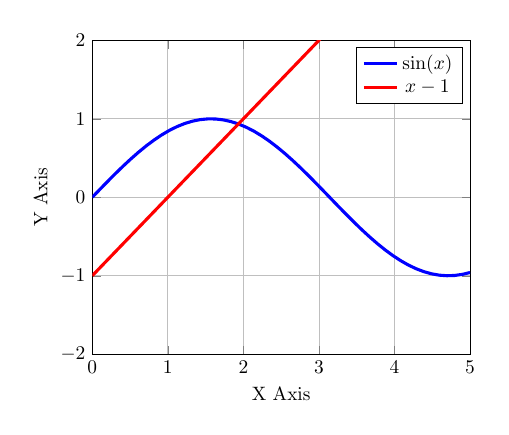
\begin{tikzpicture}[scale=0.7]
			\begin{axis}[
					xmax=5,
					xmin=0,
					ymax=2,
					ymin=-2,
					samples=50,
					grid=major,
					xlabel={X Axis},
					ylabel={Y Axis},
				]
				\addplot[blue, ultra thick,domain=0:5]{sin(deg(x))};
				\addplot[red, ultra thick,domain=0:5]{x-1};
				\legend{$\sin(x)$,$x-1$}
			\end{axis}
		\end{tikzpicture}
		\caption{Plot of the equation $\sin(x)=x-1$}
		\label{sketch:exm-continuous-opposite-signs:2}
	\end{figure}
\end{exm}

\begin{thm}\label{thm-intermediate-value-theorem}
	Let $f:[a,b]\to\mathbb{R}$ be a continuous function, and let $y_0$ be a value
	between $f(a)$ and $f(b)$. Then there exists an $x_0\in(a,b)$ such that
	\footnote{This a generalization of \pref{theorem}{thm-continuous-opposite-signs}}
	$f(x_0)=y_0$. \textit{Remark}: This theorem is also known as the intermediate
	value theorem.
\end{thm}

\begin{proof}
	Of \pref{theorem}{thm-intermediate-value-theorem}.
	\begin{flushleft}
		Assume \gls{wlog} that $f(a)<y_0<f(b)$. Then define $g(x)=f(x)-y_0$. By
		\pref{theorem}{thm-arithmetic-continuous} this function is also continuous on $[a,b]$.
		Therefore,
		\begin{align*}
			 & g(a)=f(a)-y_0<0, \\
			 & g(b)=f(b)-y_0>0
		\end{align*}
	\end{flushleft}
	By \pref{theorem}{thm-continuous-opposite-signs} there exists an $x_0$ such that
	$g(x_0)=0$. Therefore, $f(x_0)=y_0$.
\end{proof}

\begin{thm}\label{thm-weierstrass-theorems}
	Let $f:[a,b]\to\mathbb{R}$ be a continuous function. Weierstrass states the
	following two theorems:
	\begin{enumerate}
		\item The function $f$ is bounded.
		\item The function $f$ assumes a minimum and a maximum.
	\end{enumerate}
\end{thm}

\begin{thm}\label{thm-monotone-closed-interval}
	Let $f:[a,b]\to\mathbb{R}$ be a monotone function. Then, $f$ is continuous
	\textit{iff} the image of $f$ is a closed interval.
\end{thm}

\begin{proof}
	Of theorem (\ref{thm-monotone-closed-interval}).
	\begin{flushleft}
		By \pref{theorem}{thm-weierstrass-theorems}, statement 2, the function $f$
		assumes a minimum $m$ and maximum $M$. The image of $f$ is $[m,M]$ because
		$f$ obtains any value $y_0\in(m,M)$ by \pref{the intermediate value theorem}{thm-intermediate-value-theorem}.
	\end{flushleft}
\end{proof}

\begin{thm}\label{thm-continuous-monotone-invertible}
	If $f$ is continuous and strictly monotone, then $f$ is invertible whose
	inverse function is also continuous and monotone.
\end{thm}


\section{Single Variable Calculus}\label{sec-single-var-calc}

TODO: Add descriptions


\subsection{Derivatives}\label{subsec-derivatives}

\begin{definition}\label{def-differentiable}
	We say that a function $f$ is differentiable at $x_0$ if the limit in
	\pref{equation}{eq-differentiable} exists and is finite. The (first) derivative
	of $f$ at $x_0$ is equal to the result of this limit and is denoted by
	\begin{equation}\label{eq-differentiable}
		\lim_{x \to x_0}\frac{f(x)-f(x_0)}{x-x_0} \defines f^\prime(x_0) = \frac{\diff f}{\diff x}(x_0)
	\end{equation}
\end{definition}

\begin{rem}\label{rem-differentiable}
	The limit in \pref{definition}{def-differentiable} is equivalent to
	\begin{equation}\label{eq-differentiable-alt}
		f^\prime(x_0)=\lim_{h \to 0}\frac{f(x_0+h)-f(x_0)}{h}
	\end{equation}
	You can convince yourself that these definitions are equivalent by substituting
	$h\defines x-x_0$.
\end{rem}

\begin{definition}
	If $f$ is differentiable at $x_0$, then
	\begin{equation}
		y = f^\prime(x_0)(x-x_0)+f(x_0)
	\end{equation}
	is called the tangent line of $f$ at $x_0$.
\end{definition}

\begin{exm}\label{exm-derivatives:1}
	Let $f(x)=c$. For any $x_0\in\domain{f}$,
	\begin{align*}
		f^\prime(x_0) & = \lim_{x \to x_0}\frac{c-c}{x-x_0} \\
		              & = 0
	\end{align*}
\end{exm}

\begin{exm}\label{exm-derivatives:2}
	Let $f(x)=x$. For any $x_0\in\domain{f}$,
	\begin{align*}
		f^\prime(x_0) & = \lim_{x \to x_0}\frac{x-x_0}{x-x_0} \\
		              & = 1
	\end{align*}
\end{exm}

\begin{exm}\label{exm-derivatives:3}
	Let $f(x)=x^2$. For any $x_0\in\domain{f}$,
	\begin{align*}
		f^\prime(x_0) & = \lim_{x \to x_0}\frac{x^2-x_0^2}{x-x_0}      \\
		              & = \lim_{x \to x_0}\frac{(x-x_0)(x+x_0)}{x-x_0} \\
		              & = \lim_{x \to x_0} \left(x+x_0\right)          \\
		              & = 2x_0
	\end{align*}
\end{exm}

\begin{exm}\label{exm-derivatives:4}
	Let $f(x)=\sqrt{x}$. For any\footnote{This function in particular is not
		differentiable in the origin} $x_0\in\domain{f}:x_0>0$,
	\begin{align*}
		f^\prime(x_0) & = \lim_{x \to x_0}\frac{\sqrt{x}-\sqrt{x_0}}{x-x_0}                                               \\
		              & = \lim_{x \to x_0}\frac{(\sqrt{x}-\sqrt{x_0})(\sqrt{x}+\sqrt{x_0})}{(x-x_0)(\sqrt{x}+\sqrt{x_0})} \\
		              & = \lim_{x \to x_0}\frac{x-x_0}{(x-x_0)(\sqrt{x}+\sqrt{x_0})}                                      \\
		              & = \lim_{x \to x_0}\frac{1}{\sqrt{x}+\sqrt{x_0}}                                                   \\
		              & = \frac{1}{2\sqrt{x_0}}
	\end{align*}
\end{exm}

\begin{exm}\label{exm-derivatives:5}
	Let $f(x)=\sin(x)$. For any $x_0\in\domain{f}$,
	\begin{align*}
		f^\prime(x_0) & = \lim_{x \to x_0}\frac{\sin(x)-\sin(x_0)}{x-x_0}                                                                                                                                                               \\
		              & = \lim_{x \to x_0}\frac{2\sin\left(\frac{x-x_0}{2}\right)\cos\left(\frac{x+x_0}{2}\right)}{x-x_0}                                                                                                               \\
		              & = \lim_{x \to x_0}\left(\frac{\sin\left(\frac{x-x_0}{2}\right)}{\frac{x-x_0}{2}}\right)\lim_{x \to x_0}\left(\cos\left(\frac{x+x_0}{2}\right)\right) &  & \text{definition (\ref{thm-limit-arithmetic})}        \\
		              & = \cos(x_0)                                                                                                                                          &  & \text{example (\ref{exm-important-sin-over-x-limit})}
	\end{align*}
\end{exm}

\begin{rem}\label{rem-euler-limit}
	We can rewrite theorem (\ref{thm-euler-sequence-monotonicity-increasing}) as
	function, \textit{i.e.}
	\begin{equation}
		\exp(x)\defines\lim_{h \to 0}\left(1+hx\right)^\frac{1}{h}=e
	\end{equation}
\end{rem}

\begin{definition}\label{def-euler-alt}
	An alternative definition of the euler number defines that $e$ is the unique
	positive number for which $f(x_0)=\exp(x_0)$, and
	\begin{align}
		f'(x_0) & = \lim_{h\to0}\frac{f(x_0+h)-f(x_0)}{h}\nonumber                          \\
		        & = \lim_{h\to0}\frac{\exp(x_0+h)-\exp(x_0)}{h}         &  & x_0=0\nonumber \\
		        & = \lim_{h\to0}\frac{\exp(h)-1}{h}\label{eq-euler-alt}                     \\
		        & = 1\nonumber
	\end{align}
\end{definition}

\begin{exm}\label{exm-derivatives:6}
	Let $f(x)=\ln(x)$. For any $x_0\in\domain{f}$,
	\begin{align*}
		f^\prime(x_0) & = \lim_{h \to 0}\frac{\ln(x_0+h)-\ln(x_0)}{h}                                                                                                           \\
		              & = \lim_{h \to 0}\frac{\ln\left(\frac{x+h}{x_0}\right)}{h}                                                                                               \\
		              & = \ln\left(\lim_{h \to 0}\left(\left(1+\frac{h}{x_0}\right)^{\frac{1}{h}}\right)\right) &  & \text{\pref{theorem}{thm-elementary-functions-continuous}} \\
		              & = \ln\left(\exp\left(\frac{1}{x_0}\right)\right)                                        &  & \text{\pref{remark}{rem-euler-limit}}                      \\
		              & = \frac{1}{x_0}
	\end{align*}
\end{exm}

\begin{exm}\label{exm-derivatives:7}
	Let $f(x)=\abs{x}$. For $x=0$ this limit does not exists because
	\begin{align*}
		f^\prime(x_0) & = \lim_{x \to 0}\frac{\abs{x}-\abs{0}}{x-0} \\
		              & = \lim_{x \to 0}\frac{\abs{x}}{x}
	\end{align*}
	but notice that this limit doesn't exists since
	\begin{equation*}
		\lim_{x \to 0^+}\frac{x}{x} = 1 \neq -1 = \lim_{x \to 0^-}\frac{-x}{x}
	\end{equation*}
	wherefore the derivative of the absolute value function \gls{dne} in the origin.
\end{exm}

\begin{rem}
	In \pref{example}{exm-derivatives:6} we saw why functions are not differentiable
	at cusps.
\end{rem}

\begin{thm}\label{thm-differentiability-implies-continuity}
	If the function $f$ is differentiable at $x_0$, then $f$ is continuous at $x_0$.
\end{thm}

\begin{proof}
	Of \pref{theorem}{thm-differentiability-implies-continuity}.
	\begin{flushleft}
		One of the prerequisites of this theorem are that the limit stated in
		\pref{definition}{def-differentiable} exists. Therefore,
		\begin{align*}
			\lim_{x \to x_0}\left(f(x)-f(x_0)\right) & = \underbrace{\lim_{x \to x_0}\left(\frac{f(x)-f(x_0)}{x-x_0}\right)}_{=f^\prime(x_0)}\cdot\underbrace{\lim_{x \to x_0}(x-x_0)}_{=0}                                                     \\
			                                         & =  0                                                                                                                                 &  & \text{\pref{definition}{thm-limit-arithmetic}} \\
		\end{align*}
		But this means $f(x)\tolim{x}{x_0}0$.
		So, by \pref{definition}{def-continuity-at-point-a}, $f$ is continuous at
		the point $x_0$.
	\end{flushleft}
\end{proof}

\begin{rem}\label{rem-continuity-doesnt-imply-differentiability}
	It is very important to point out that the converse of \pref{theorem}{thm-differentiability-implies-continuity}
	is false, \textit{i.e.} continuity does not imply differentiability. See \pref{example}{exm-derivatives:6}
	why this couldn't possibly be true. However, if $f$ is not continuous, then $f$ is not differentiable, either.
\end{rem}

\begin{definition}\label{def-one-sided-derivatives}
	Similar to \pref{definition}{def-differentiable}, we can define one-sided derivatives by
	\begin{equation}\label{eq-right-sided-derivative}
		f_+^\prime(x)=\lim_{x \to x_0^+}\frac{f(x)-f(x_0)}{x-x_0}
	\end{equation}
	\begin{equation}\label{eq-left-sided-derivative}
		f_-^\prime(x)=\lim_{x \to x_0^-}\frac{f(x)-f(x_0)}{x-x_0}
	\end{equation}
	if the limit exists.
\end{definition}

\begin{thm}\label{thm-derivative-arithmetic}
	Let $f$ and $g$ be two differentiable functions, and $c\in\mathbb{R}$. Then
	\begin{enumerate}
		\item $(c\cdot f)^\prime(x_0) = c \cdot f^\prime(x_0)$
		\item $(f \pm g)^\prime(x_0) = f^\prime(x_0) \pm g^\prime(x_0)$
		\item $(f \cdot g)^\prime(x_0) = f^\prime(x_0) \cdot g(x_0) + g^\prime(x_0) \cdot f(x_0)$
		\item $\left(\tfrac{f}{g}\right)^\prime(x_0) = \tfrac{f^\prime(x_0)\cdot g(x_0) - g^\prime(x_0) \cdot f(x_0)}{g^2(x_0)}$ if $g(x_0)\neq0$
	\end{enumerate}
\end{thm}

\begin{proof}
	Of \pref{theorem}{thm-derivative-arithmetic}.
	\begin{flushleft}
		\textbf{Product Rule}:
		\begin{align*}
			(f \cdot g)^\prime(x_0) & = \lim_{h \to 0}\frac{f(x_0+h) g(x_0+h)-f(x_0) g(x_0)}{h}                                                           \\
			                        & = \lim_{h \to 0}\left(\frac{1}{h}\big( f(x_0+h) g(x_0+h) - f(x_0)(x_0+h) +f(x_0)(x_0+h) - f(x_0) g(x_0)\big)\right) \\
			                        & = \lim_{h \to 0}\left(g(x_0+h)\frac{f(x_0+h)-f(x_0)}{h}+f(x_0)\frac{g(x_0+h)-g(x_0)}{h}\right)                      \\
			                        & = g(x_0) \cdot f^\prime(x_0) + f(x_0) \cdot g^\prime(x_0)
		\end{align*}
		Notice that in the last step we used the fact that by \pref{theorem}{thm-differentiability-implies-continuity},
		$g$ is continuous which is an important detail required in this proof that explains why
		$g(x_0+h)\tolim{h}{0}g(x_0)$.
	\end{flushleft}
\end{proof}

\begin{thm}\label{thm-chain-rule}
	If $f$ is differentiable at $x_0$ and $g$ is differentiable at $f(x_a)$, then
	\begin{equation}\label{eq-chain-rule}
		(g \circ f)^\prime(x_0) = \underbrace{g^\prime(f(x_0))}_{\text{outer derivative}} \cdot \underbrace{f^\prime(x_0)}_{\text{inner derivative}}
	\end{equation}
	This is called the chain rule.
\end{thm}

\begin{thm}\label{thm-derivative-of-inverse-function}
	Let $y=f(x)$ be invertible, continuous at a neighborhood of $x_0$, and differentiable
	at $x_0$. Also assume that $f^\prime(x_0)\neq0$. Then $x=f^{-1}(y)$ is differentiable
	at $y_0=f(x_0)$, and
	\begin{equation}\label{eq-derivative-of-inverse-function}
		\left(f^{-1}\right)^\prime(y_0)=\frac{1}{f^\prime(x_0)}
	\end{equation}
\end{thm}

\begin{exm}\label{exm-derivative-of-inverse-function:1}
	We know that for all $x>0$, $(\ln(x))^\prime=\tfrac{1}{x}$. The inverse function
	of $y=\ln(x)$ is $x=e^y$. Hence, by \pref{theorem}{thm-derivative-of-inverse-function}
	we can write
	\begin{equation*}
		(e^y)^\prime = \frac{1}{\ln(x)^\prime} = \frac{1}{x^{-1}} = e^y
	\end{equation*}
	where we used the result obtained from \pref{example}{exm-derivatives:5}.
\end{exm}

\begin{exm}\label{exm-derivative-of-inverse-function:2}
	Let $f(x)=\sin(x)=y$ and $f^{-1}(x)=\arcsin(y)$. Hence, by
	\pref{theorem}{thm-derivative-of-inverse-function} we can write
	\begin{align*}
		(\arcsin(y))^\prime & = \frac{1}{\sin(x)^\prime}     \\
		                    & = \frac{1}{\cos(x)}            \\
		                    & = \frac{1}{\sqrt{1-\sin^2(x)}} \\
		                    & = \frac{1}{\sqrt{1-y^2}}
	\end{align*}
\end{exm}

\begin{exm}\label{exm-derivative-of-inverse-function:3}
	Let $f(x)=\tan(x)=y$ and $f^{-1}(x)=\arctan(y)$. Hence, by
	\pref{theorem}{thm-derivative-of-inverse-function} we can write TODO
\end{exm}

\begin{rem}\label{rem-first-derivative-polynomial}
	Let $f(x)=x^\alpha$ with $\alpha\in\mathbb{R}$ and $x>0$. Define
	$g(x)\defines \ln(f(x))$. By using the chain rule we get that
	\begin{equation}\label{eq-first-derivative-polynomial:1}
		g^\prime(x) = \frac{1}{f(x)} \cdot f^\prime(x)
	\end{equation}
	On the other hand,
	\begin{equation}\label{eq-first-derivative-polynomial:2}
		g(x) = \ln(x^\alpha) = \alpha\ln(x) \implies g^\prime(x) = \frac{\alpha}{x}
	\end{equation}
	So by \pref{equation}{eq-first-derivative-polynomial:1} and \pref{equation}{eq-first-derivative-polynomial:2},
	\begin{align*}
		\frac{1}{f(x)} \cdot f^\prime(x) = \frac{\alpha}{x} \implies f^\prime(x) = \alpha \cdot x^{\alpha-1}
	\end{align*}
\end{rem}


\section{Appendix}\label{sec-appendix}

\begin{figure}[ht]
    \centering
    \caption{Various plots for $f(x)=x^2-1$ from example (\ref{exm-injective-surjective-bijective})}
    \label{sktech:exm-1:4}
    \begin{subfigure}[ht]{0.47\textwidth}
        \centering
        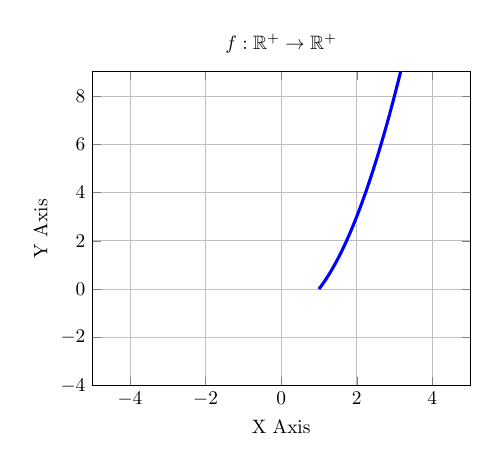
\begin{tikzpicture}[scale=0.7]
            \begin{axis}[
                xmax=5,
                xmin=-5,
                ymax=9,
                ymin=-4,
                samples=50,
                grid=major,
                xlabel={X Axis},
                ylabel={Y Axis},
                title={$f:\mathbb{R}^+\rightarrow\mathbb{R}^+$}
            ]
            \addplot[blue,ultra thick,domain=1:5](x,x^2-1);
        \end{axis}
        \end{tikzpicture}
        \label{sketch:exm-1}
    \end{subfigure}
    \hfill
    \begin{subfigure}[ht]{0.47\textwidth}
        \centering
        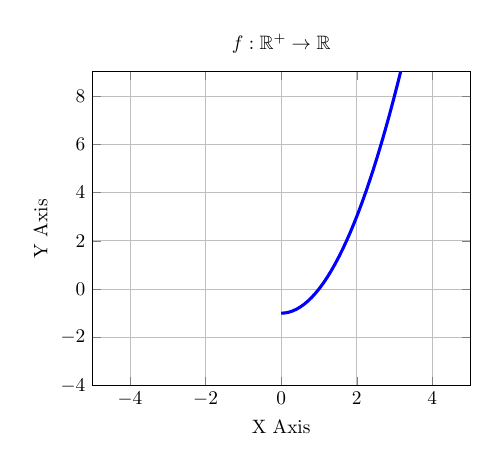
\begin{tikzpicture}[scale=0.7]
            \begin{axis}[
                xmax=5,
                xmin=-5,
                ymax=9,
                ymin=-4,
                samples=50,
                grid=major,
                xlabel={X Axis},
                ylabel={Y Axis},
                title={$f:\mathbb{R}^+\rightarrow\mathbb{R}$}
            ]
            \addplot[blue,ultra thick,domain=0:5](x,x^2-1);
        \end{axis}
        \end{tikzpicture}
        \label{sketch:exm-2}
    \end{subfigure}
    \vfill
    \begin{subfigure}[ht]{0.47\textwidth}
        \centering
        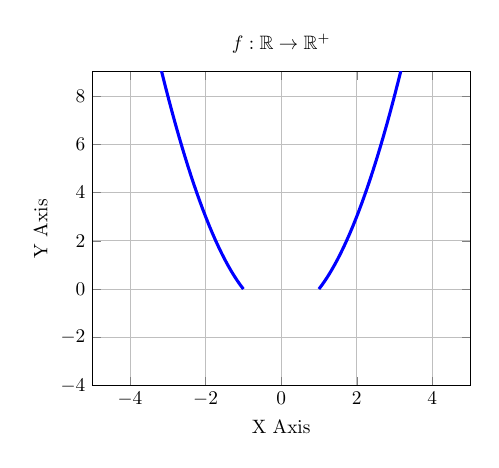
\begin{tikzpicture}[scale=0.7]
            \begin{axis}[
                xmax=5,
                xmin=-5,
                ymax=9,
                ymin=-4,
                samples=50,
                grid=major,
                xlabel={X Axis},
                ylabel={Y Axis},
                title={$f:\mathbb{R}\rightarrow\mathbb{R}^+$}
            ]
            \addplot[blue,ultra thick,domain=-5:-1](x,x^2-1);
            \addplot[blue,ultra thick,domain=1:5](x,x^2-1);
        \end{axis}
        \end{tikzpicture}
        \label{sketch:exm-3}
    \end{subfigure}
    \hfill
    \begin{subfigure}[ht]{0.47\textwidth}
        \centering
        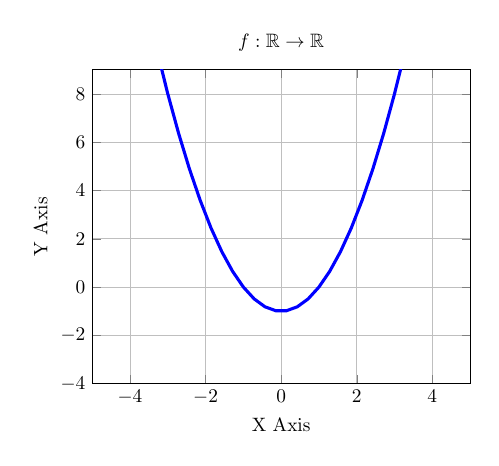
\begin{tikzpicture}[scale=0.7]
            \begin{axis}[
                xmax=5,
                xmin=-5,
                ymax=9,
                ymin=-4,
                samples=50,
                grid=major,
                xlabel={X Axis},
                ylabel={Y Axis},
                title={$f:\mathbb{R}\rightarrow\mathbb{R}$}
            ]
            \addplot[blue, ultra thick,domain=-5:9](x,x^2-1);
        \end{axis}
        \end{tikzpicture}
        \label{sketch:exm-4}
    \end{subfigure}
\end{figure}


% === End Section Includes ====

\newpage

\medskip
\printbibliography

\end{document}
